
The original study provides graphical results for three scenarios only: the
no-control case, the non-optimised PI-ALINEA controller, and the RL agent,
all evaluated under the base demand profile. A robustness analysis is
additionally presented for the RL agent under five levels of additive white
noise on the traffic demand (standard deviation of 50, 100, 150, 200, and
250\,veh/h). No quantitative performance indicators of any kind are reported
in the original work.

In this replication, all controllers were evaluated under the base demand
scenario as well as under each of the five noise levels, enabling a
systematic cross-controller comparison that was absent from the original
study. The quantitative performance indicators recorded for each scenario
are summarised in Table~\ref{tab:indicators}.

\begin{table}[h]
\centering
\caption{Performance indicators recorded for each controller and demand
scenario.}
\label{tab:indicators}
\begin{tabular}{ll}
\hline
\textbf{Indicator} & \textbf{Description} \\
\hline
VKT & Vehicle-kilometres travelled \\
VHT & Vehicle-hours travelled (mainline only) \\
VHT\textsubscript{queue} & Vehicle-hours travelled including ramp queue delay \\
$\bar{v}$ & Average speed, mainline only \\
$\bar{v}_\text{queue}$ & Average speed including ramp queue delay \\
Episode reward & Cumulative reward following Eq.~\ref{eq:reward_function} \\
\hline
\end{tabular}
\end{table}

A complete overview of all recorded performance values across controllers
and demand scenarios is provided in Table~\ref{tab:full_results}. Table~\ref{tab:rankings} reports the percentage gaps between controllers, which is computed relative to the best controller for each metric and demand scenario; the calculation procedure is given in the Appendix (\ref{sec:a-controll_perf}). These tables constitute the main quantitative
contribution of this replication and are discussed in detail in the
following subsections.

%% ──────────────────────────────────────────────────────────────────────
\subsection{Reproducing Baseline Results}

\subsubsection{No-Control Scenario}

Figure~\ref{fig:comparison_no_control_control_cell_density} shows the
reproduced control-cell density alongside the corresponding result reported
in the original study. Figures~\ref{fig:comparison_no_control_space_time}
and~\ref{fig:no_control_space_time_raw} present the reproduced space--time
density contours in smoothed and non-smoothed form respectively. The comparisons in
Figures~\ref{fig:comparison_no_control_control_cell_density}
and~\ref{fig:comparison_no_control_space_time} were used to fine-tune the
traffic demand profile and CTM parameters, and show a strong overall
resemblance to the original results, confirming that the simulation
environment has been reconstructed faithfully. Figure~\ref{fig:no_control_space_time_raw}
provides a direct view of the underlying simulation output without
post-processing, which is absent from the original study. Raw density
contours are preferred for reproducibility purposes, as smoothing
operations are difficult to replicate exactly and may obscure differences
between results.

\begin{figure}[htbp]
    \centering
    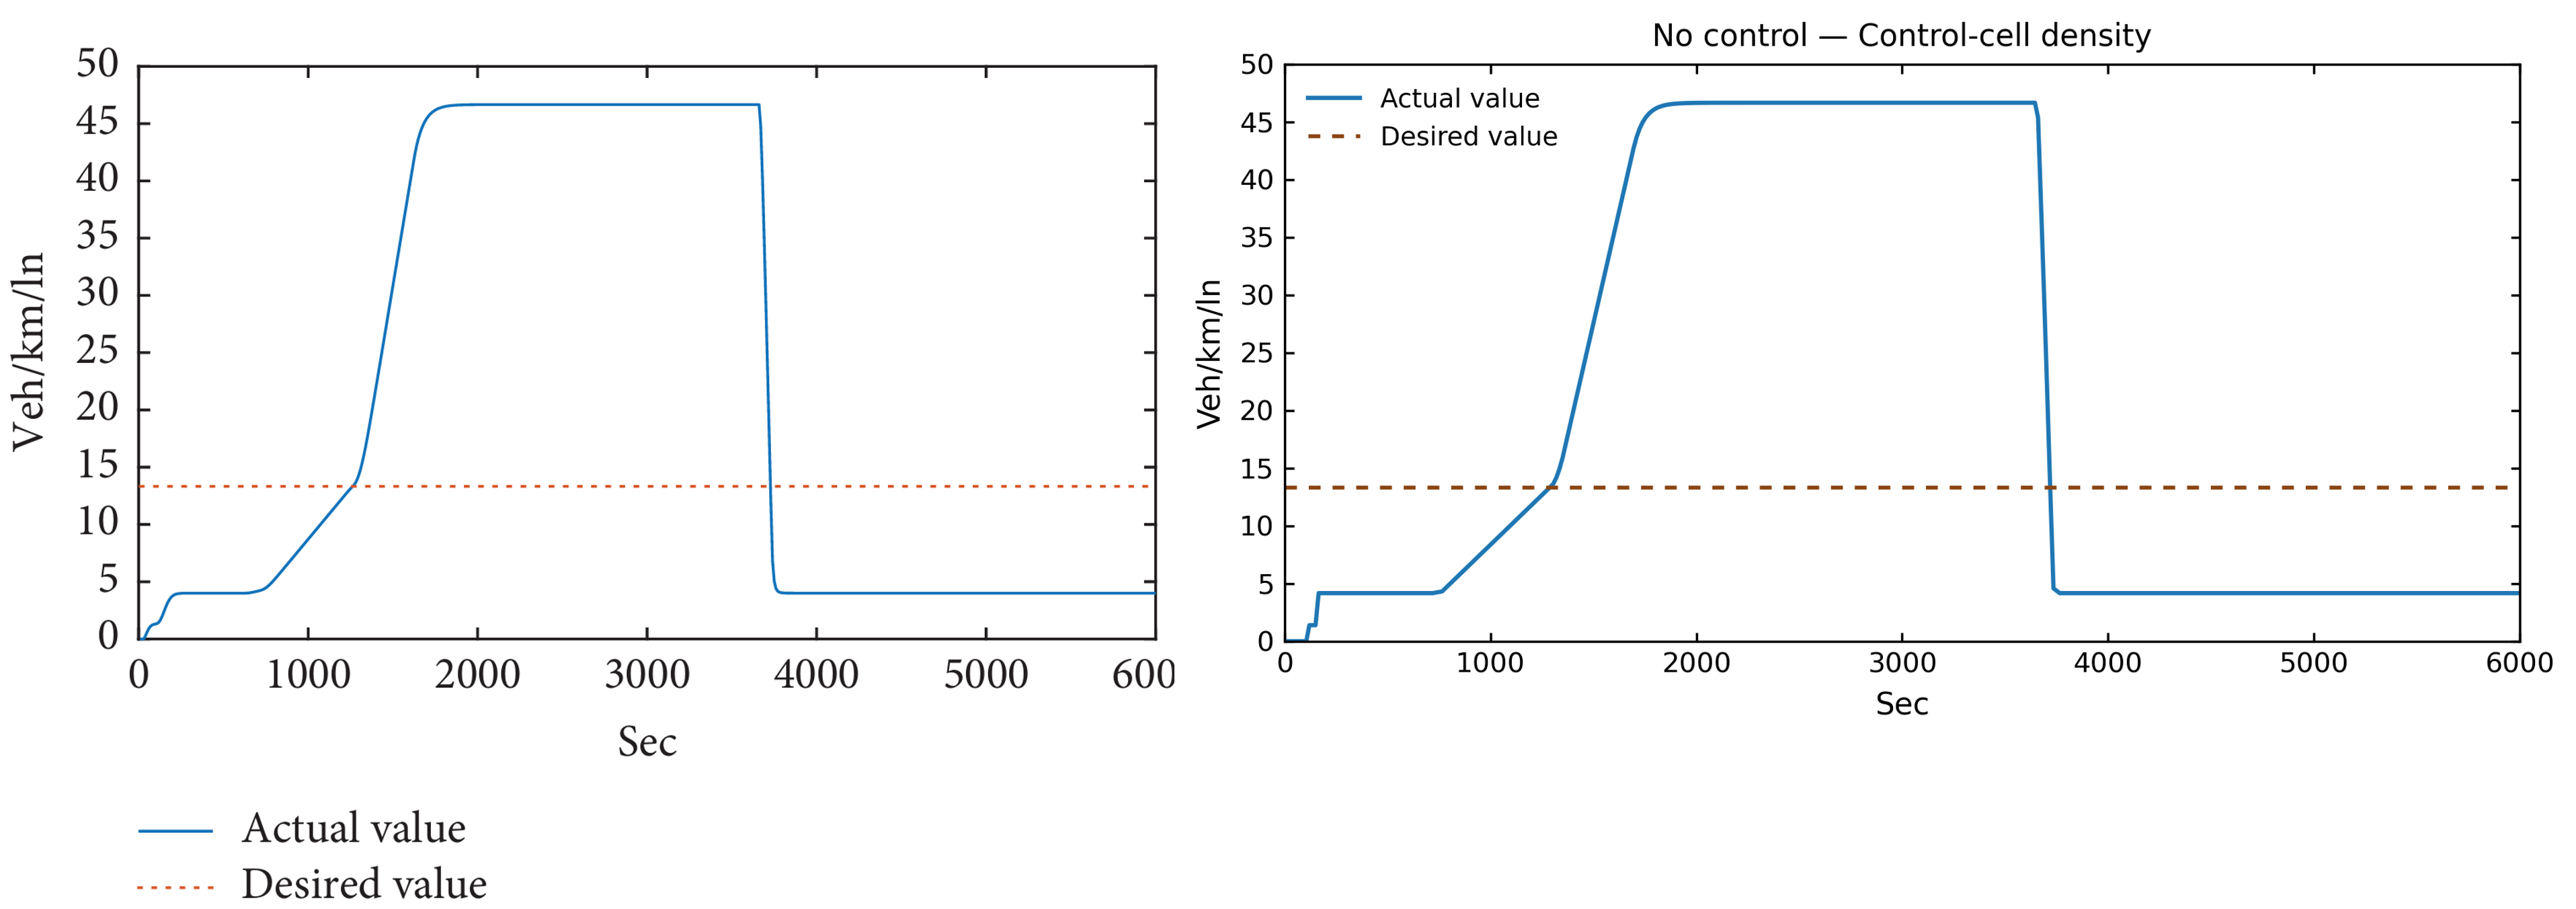
\includegraphics[width=\linewidth]{figures/No_Control_scenario/02_control_cell_density_comparison.png}
    \caption{No-control scenario: control-cell density. Original study
    (left) and reproduced result (right).}
    \label{fig:comparison_no_control_control_cell_density}
\end{figure}

\begin{figure}[htbp]
    \centering
    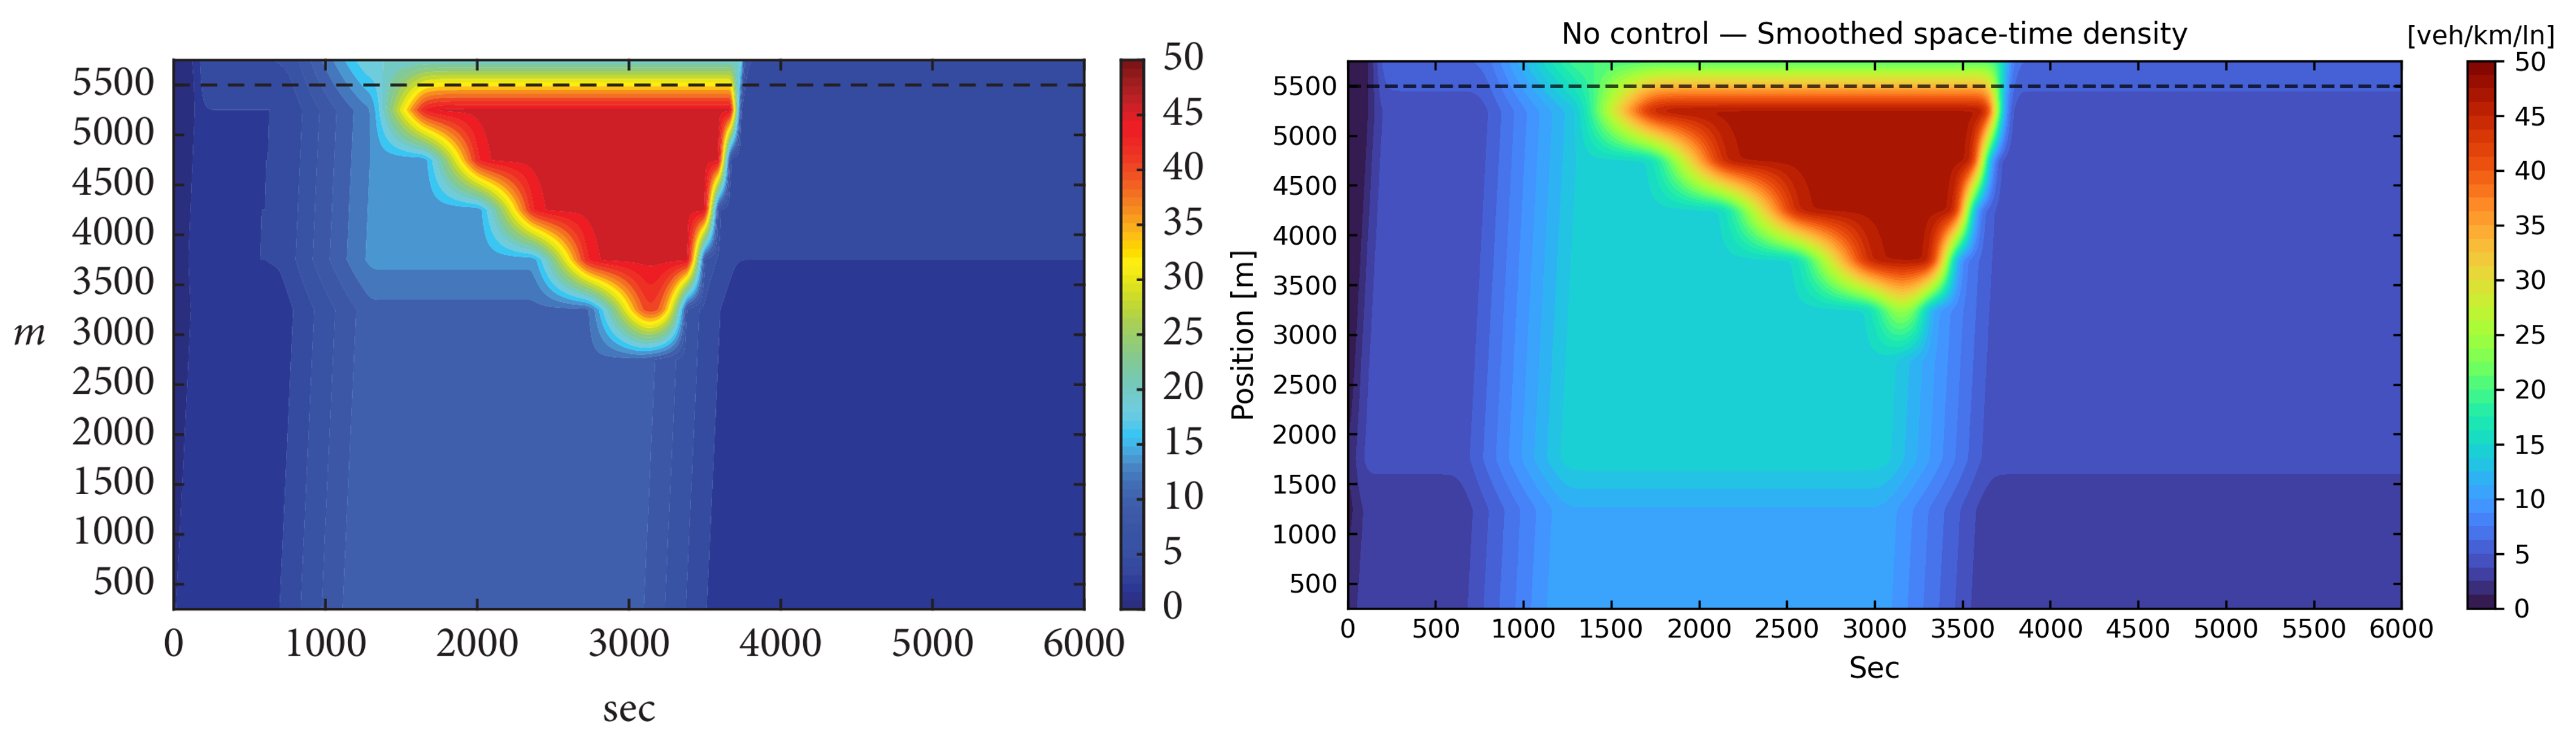
\includegraphics[width=\linewidth]{figures/No_Control_scenario/04_control_density_space_time_smoothed_comparison.png}
    \caption{No-control scenario: smoothed space--time traffic density.
    Original study (left) and reproduced result (right).}
    \label{fig:comparison_no_control_space_time}
\end{figure}

\begin{figure}[H]
    \centering
    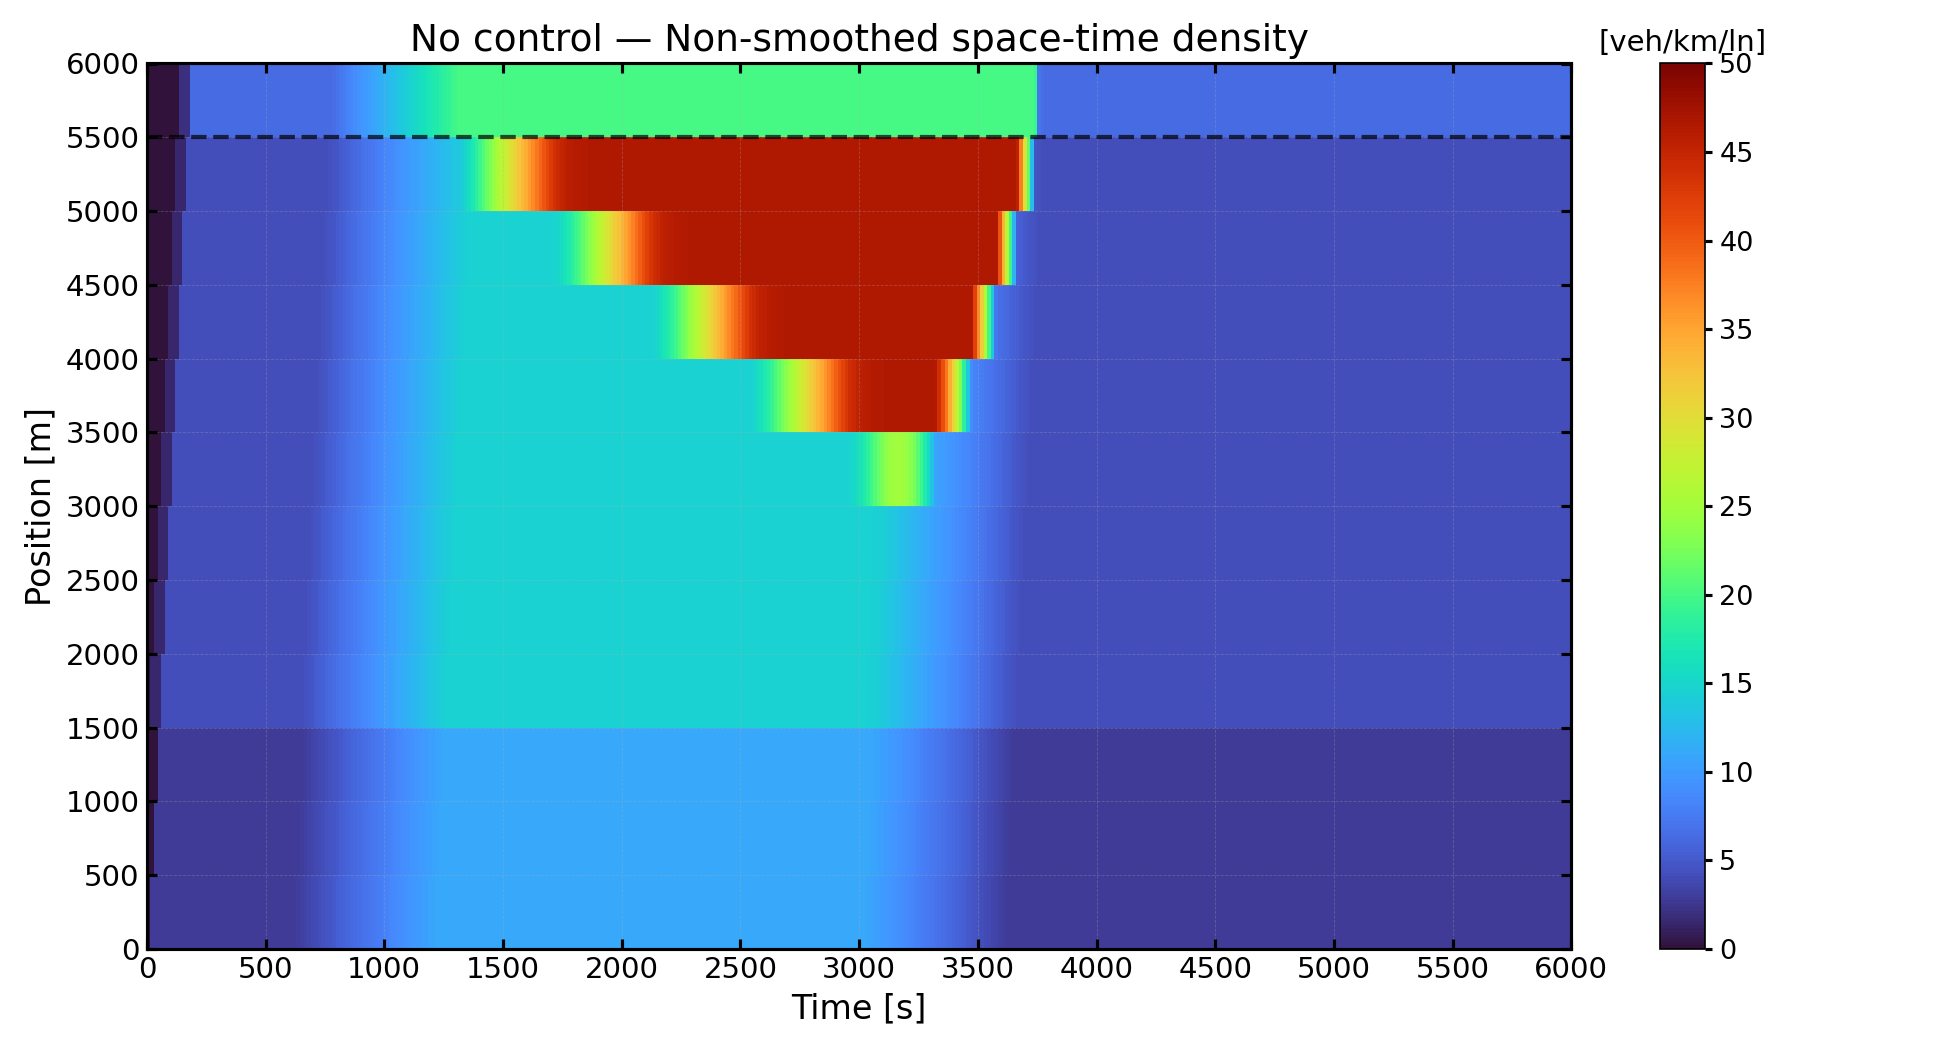
\includegraphics[width=0.4\linewidth]{figures/No_Control_scenario/03_density_space_time_raw.png}
    \caption{No-control scenario: non-smoothed space--time traffic density
    of the reproduced result.}
    \label{fig:no_control_space_time_raw}
\end{figure}

\subsubsection{PI-ALINEA Scenario}

Figures~\ref{fig:pi_alinea_original_density_space_time_smoothed},
\ref{fig:pi_alinea_original_control_cell_density},
and~\ref{fig:pi_alinea_original_metering_rate} compare the reproduced
PI-ALINEA results against those reported in the original study for the
space--time density contour, the control-cell density trajectory, and the
ramp metering rate respectively. The parameters used are those adopted
from the reference study: $K_R = 4$ and $K_P = 100$
\citep{PI-ALINEA}.

All three figures show close agreement with the original results. In
particular, the oscillatory pattern of the metering rate and the
characteristic suppression of congestion at the bottleneck are well
reproduced. Minor discrepancies in the smoothed density contours are
attributed to differences in the post-processing procedure, which was
not described in the original study. These results confirm that the
PI-ALINEA controller has been correctly implemented and that the
simulation environment produces consistent outputs under controlled
conditions.

\begin{figure}[htbp]
    \centering
    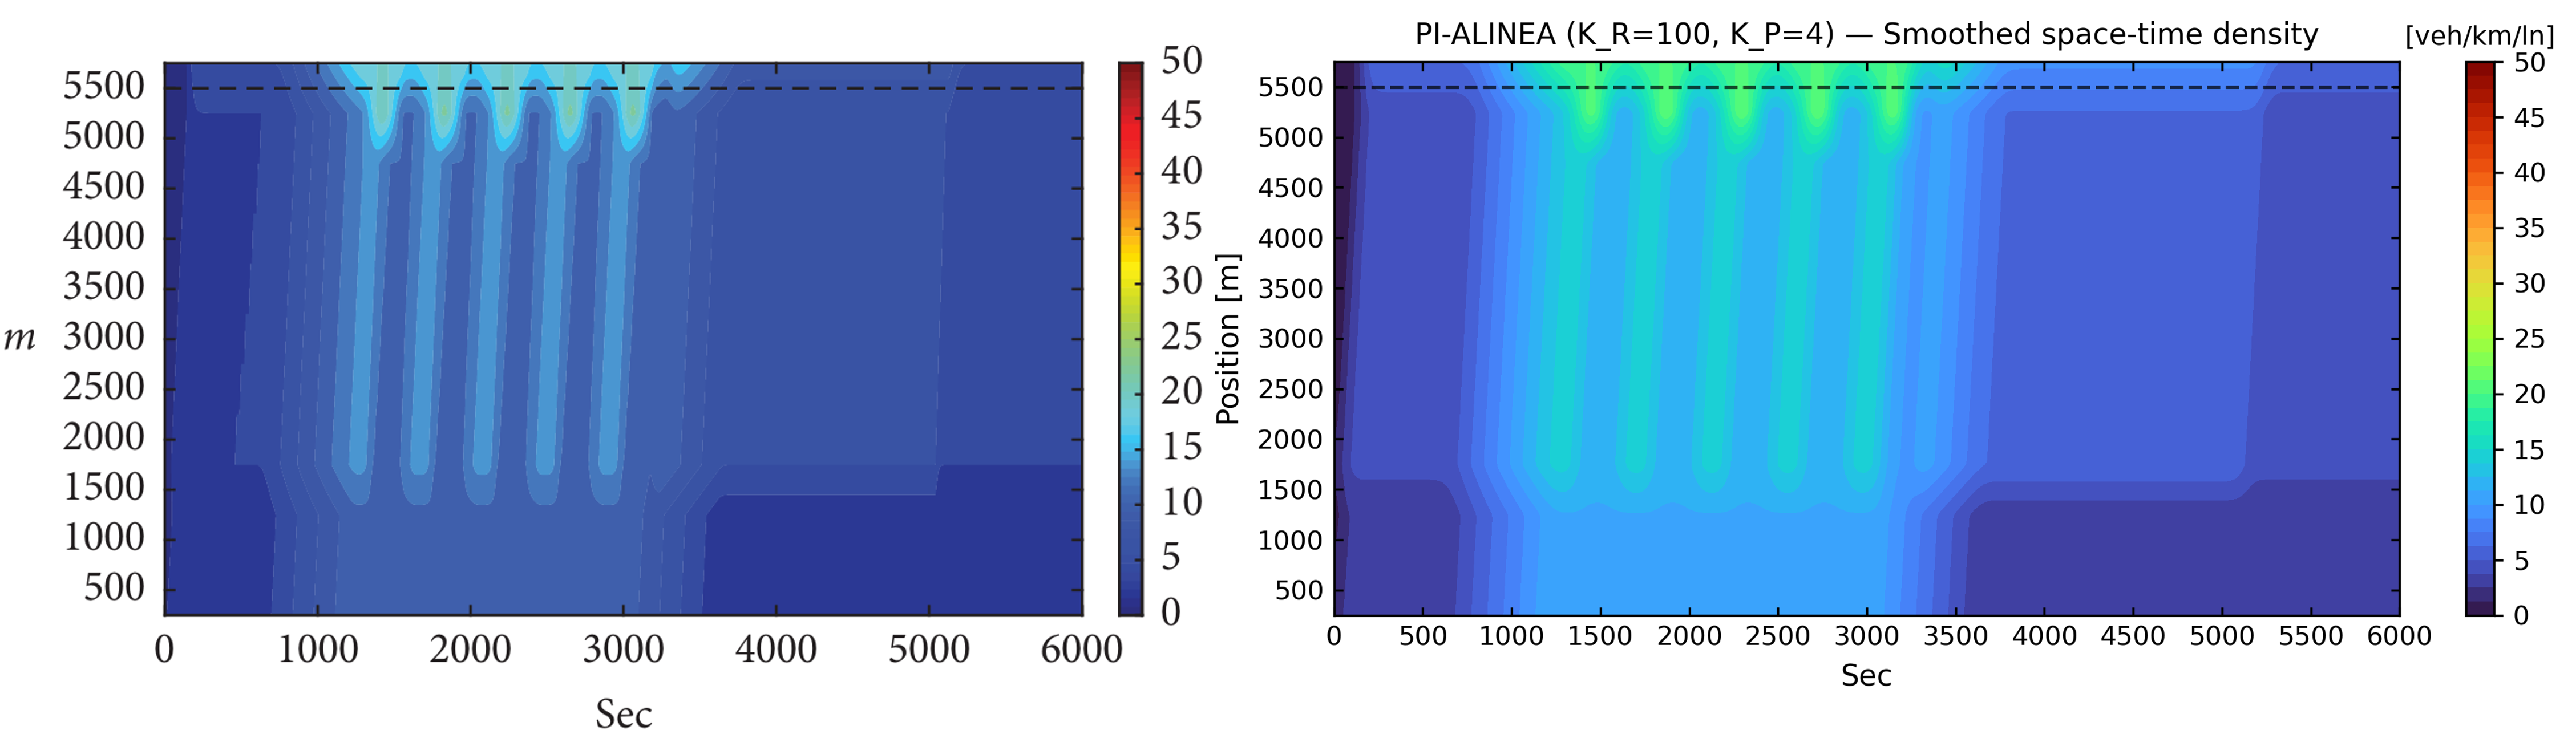
\includegraphics[width=\linewidth]{figures/PI_ALINEA/ORIGINAL/PI_alinea_base_space_time_density.png}
    \caption{Base PI-ALINEA scenario: smoothed space--time traffic density.
    Original study (left) and reproduced result (right).}
    \label{fig:pi_alinea_original_density_space_time_smoothed}
\end{figure}

\begin{figure}[htbp]
    \centering
    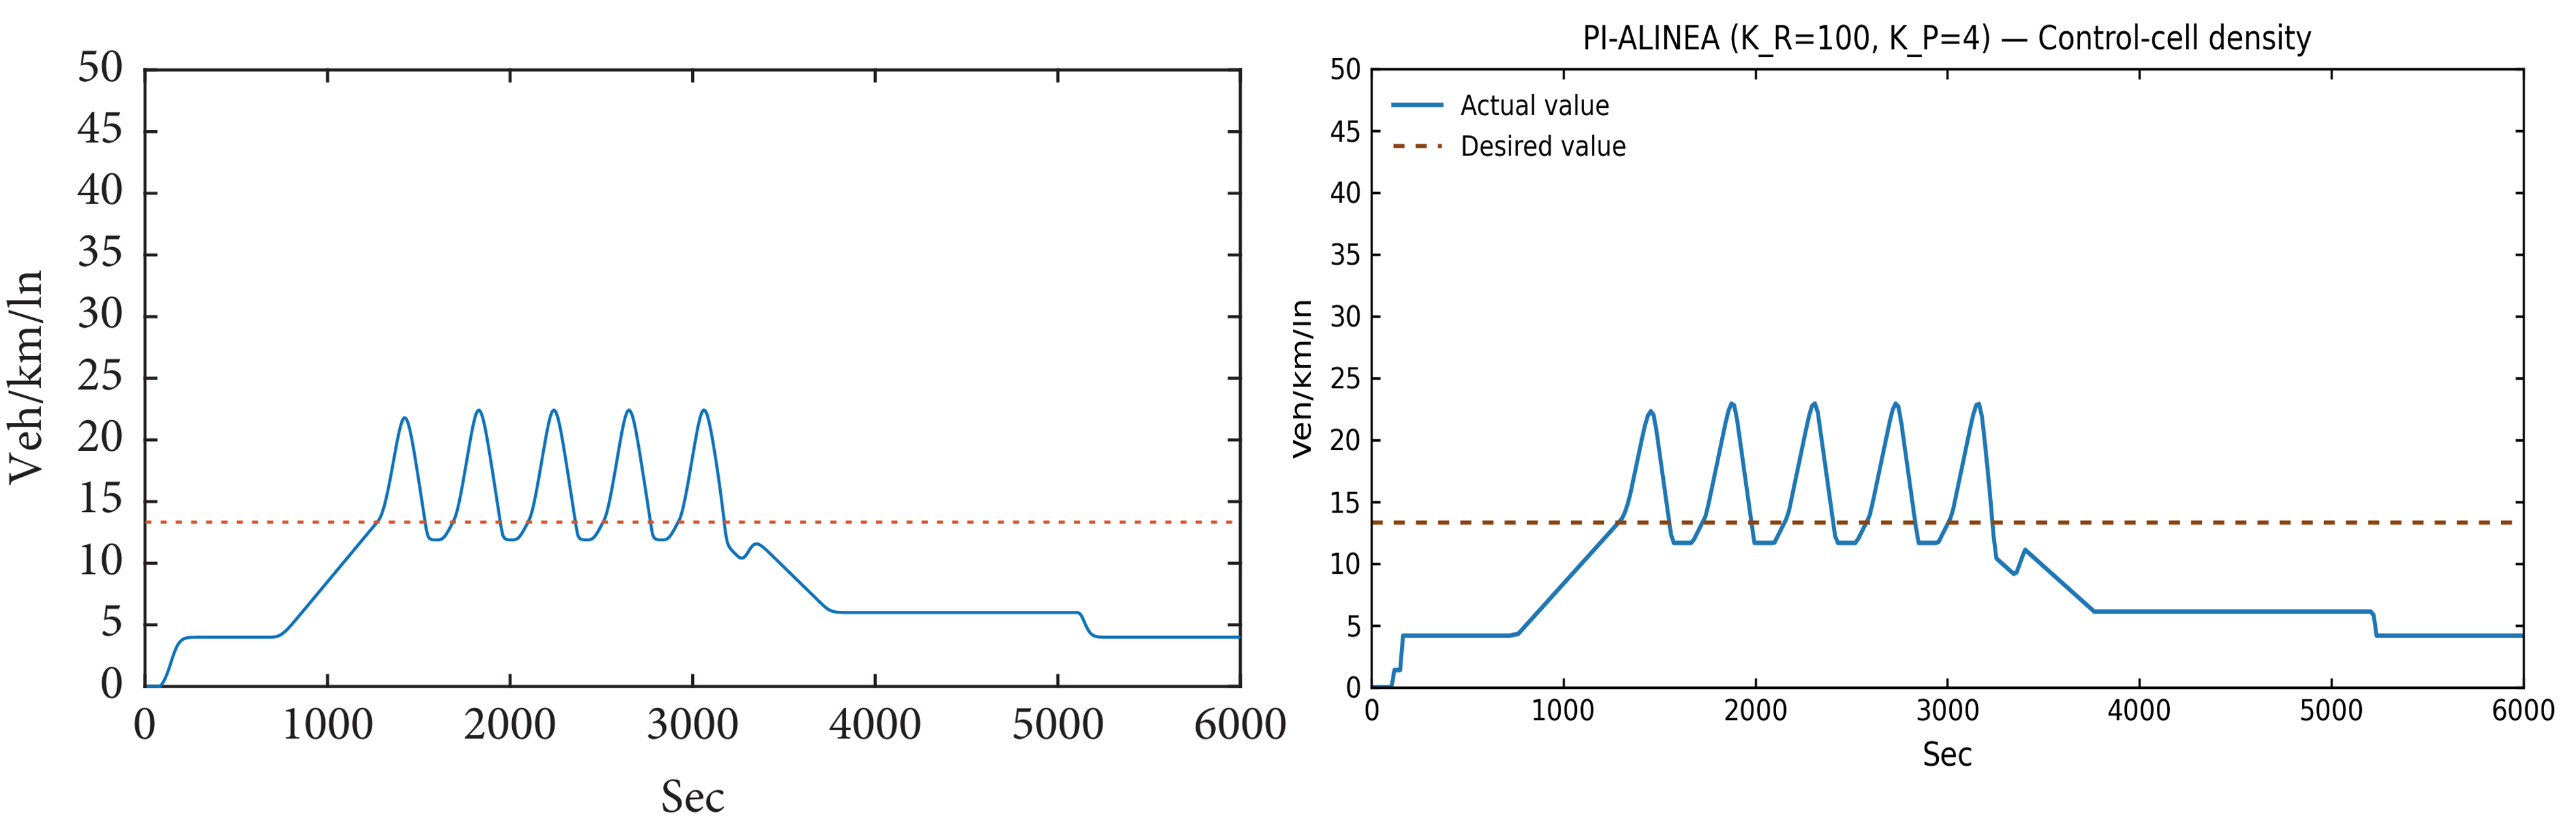
\includegraphics[width=\linewidth]{figures/PI_ALINEA/ORIGINAL/PI_alinea_base_control_cell_density.png}
    \caption{Base PI-ALINEA scenario: control-cell density. Original study
    (left) and reproduced result (right).}
    \label{fig:pi_alinea_original_control_cell_density}
\end{figure}

\begin{figure}[htbp]
    \centering
    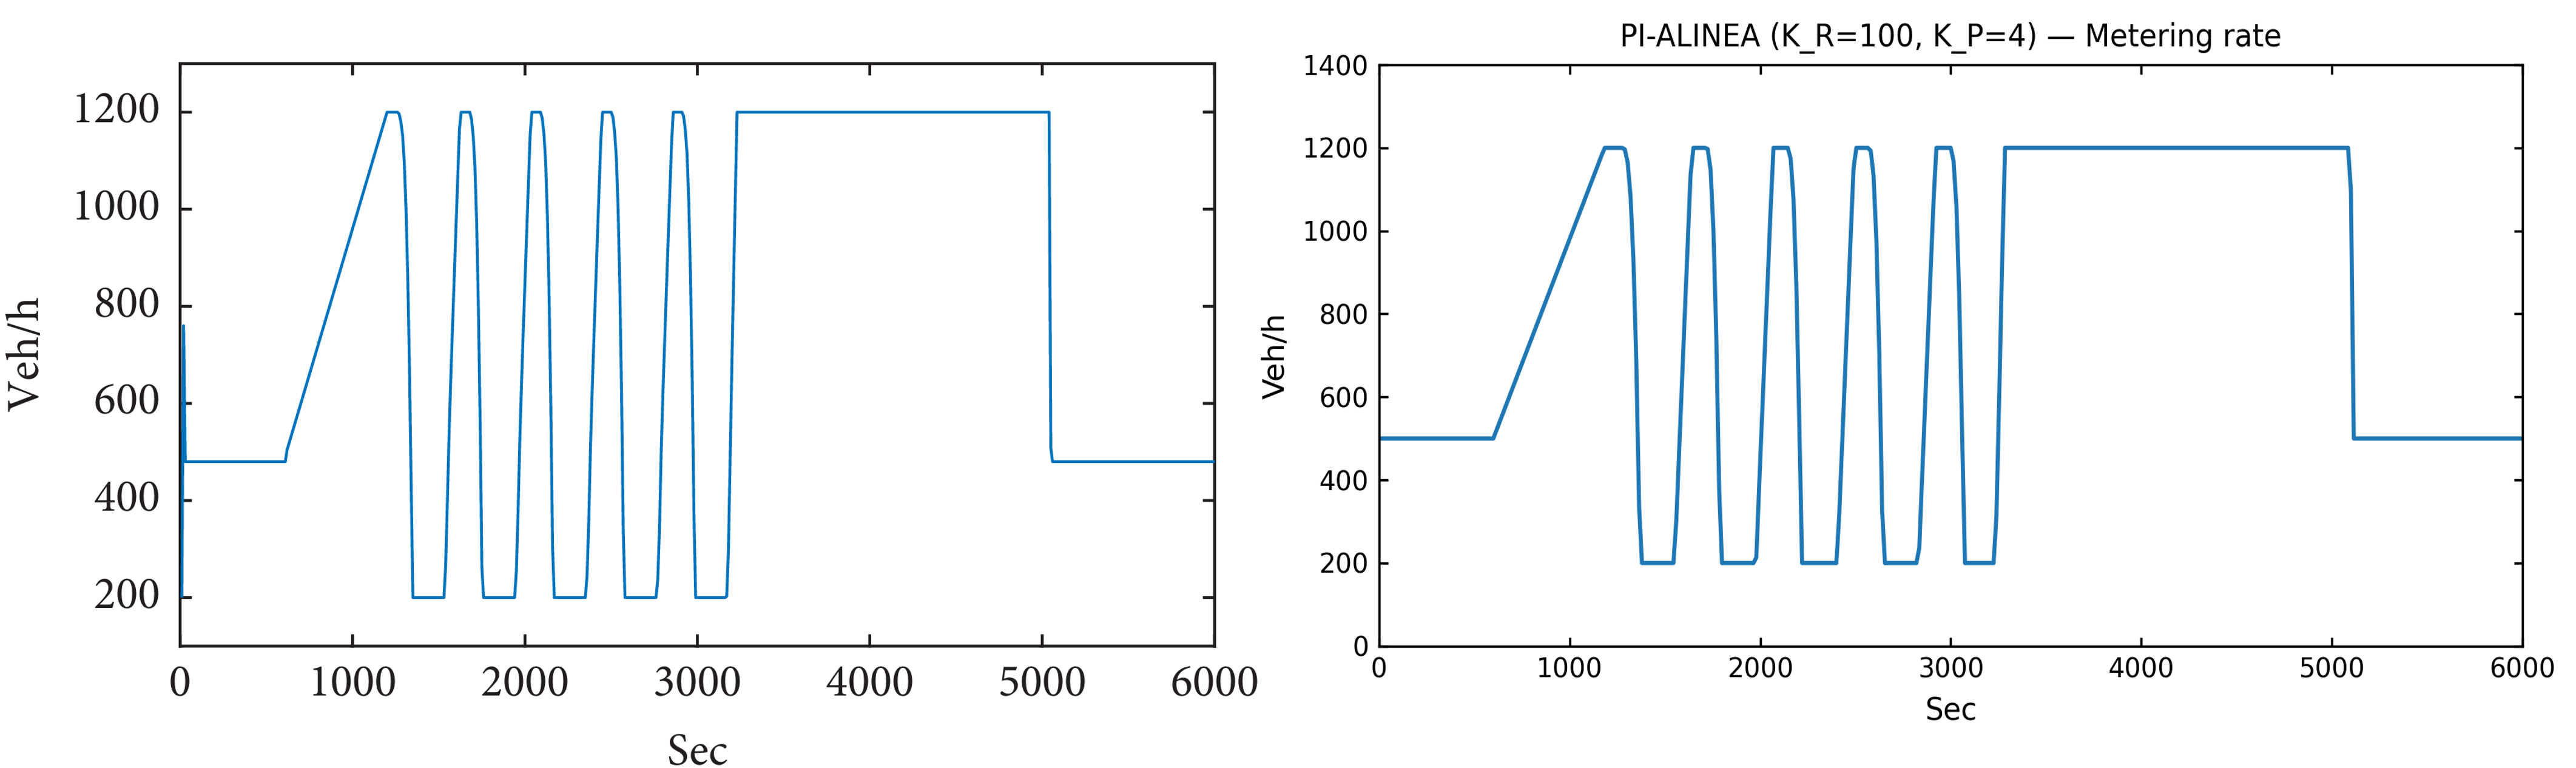
\includegraphics[width=\linewidth]{figures/PI_ALINEA/ORIGINAL/PI_alinea_base_metering_rate.png}
    \caption{Base PI-ALINEA scenario: on-ramp metering rate. Original
    study (left) and reproduced result (right).}
    \label{fig:pi_alinea_original_metering_rate}
\end{figure}

%% ──────────────────────────────────────────────────────────────────────
\subsection{Optimizing Benchmark Controllers}

The grid search identified the following optimal parameter configurations.
For PI-ALINEA, the best parameters under the mainline criterion
$\bar{v}$ were $K_R = 2$ and $K_P = 93$, yielding
$\bar{v} = 119.85\,\mathrm{km/h}$. Optimizing instead for the
queue-aware criterion $\bar{v}_\text{queue}$ produced $K_R = 2$ and
$K_P = 56$, with $\bar{v}_\text{queue} = 78.90\,\mathrm{km/h}$. For
ALINEA, the optimal gain under $\bar{v}$ was $K_R = 23$
($\bar{v} = 119.37\,\mathrm{km/h}$), and under $\bar{v}_\text{queue}$
was $K_R = 21$ ($\bar{v}_\text{queue} = 72.70\,\mathrm{km/h}$). The
similarity of the optimal $K_R$ values between the two criteria for
both controllers suggests that the integral gain plays a secondary role
relative to $K_P$ in PI-ALINEA, and that performance is relatively
robust to small variations in $K_R$ for ALINEA.

The optimised controllers can first be evaluated graphically, following the
methodology of the original study, using
Figures~\ref{fig:placeholder_opt_spacetime},
\ref{fig:placeholder_opt_control_cell}, and~\ref{fig:placeholder_opt_metering},
which show the space--time density contours, control-cell density trajectories,
and ramp metering rates under the base demand scenario.

Overall, the graphical comparison suggests that all optimised benchmark
controllers improve upon the non-optimised PI-ALINEA baseline. The improvement
is most visible in the metering-rate trajectories shown in
Figure~\ref{fig:placeholder_opt_metering}, where the optimised controllers
produce substantially more stable ramp inflows than the oscillatory metering
pattern obtained with the reference PI-ALINEA parameters in
Figure~\ref{fig:pi_alinea_original_metering_rate}. This effect is particularly
clear for the optimised PI-ALINEA configurations, whose metering rates vary more
smoothly while still preventing severe congestion at the downstream bottleneck.


\begin{figure}[htbp]
    \centering

    \begin{subfigure}{0.48\textwidth}
        \centering
        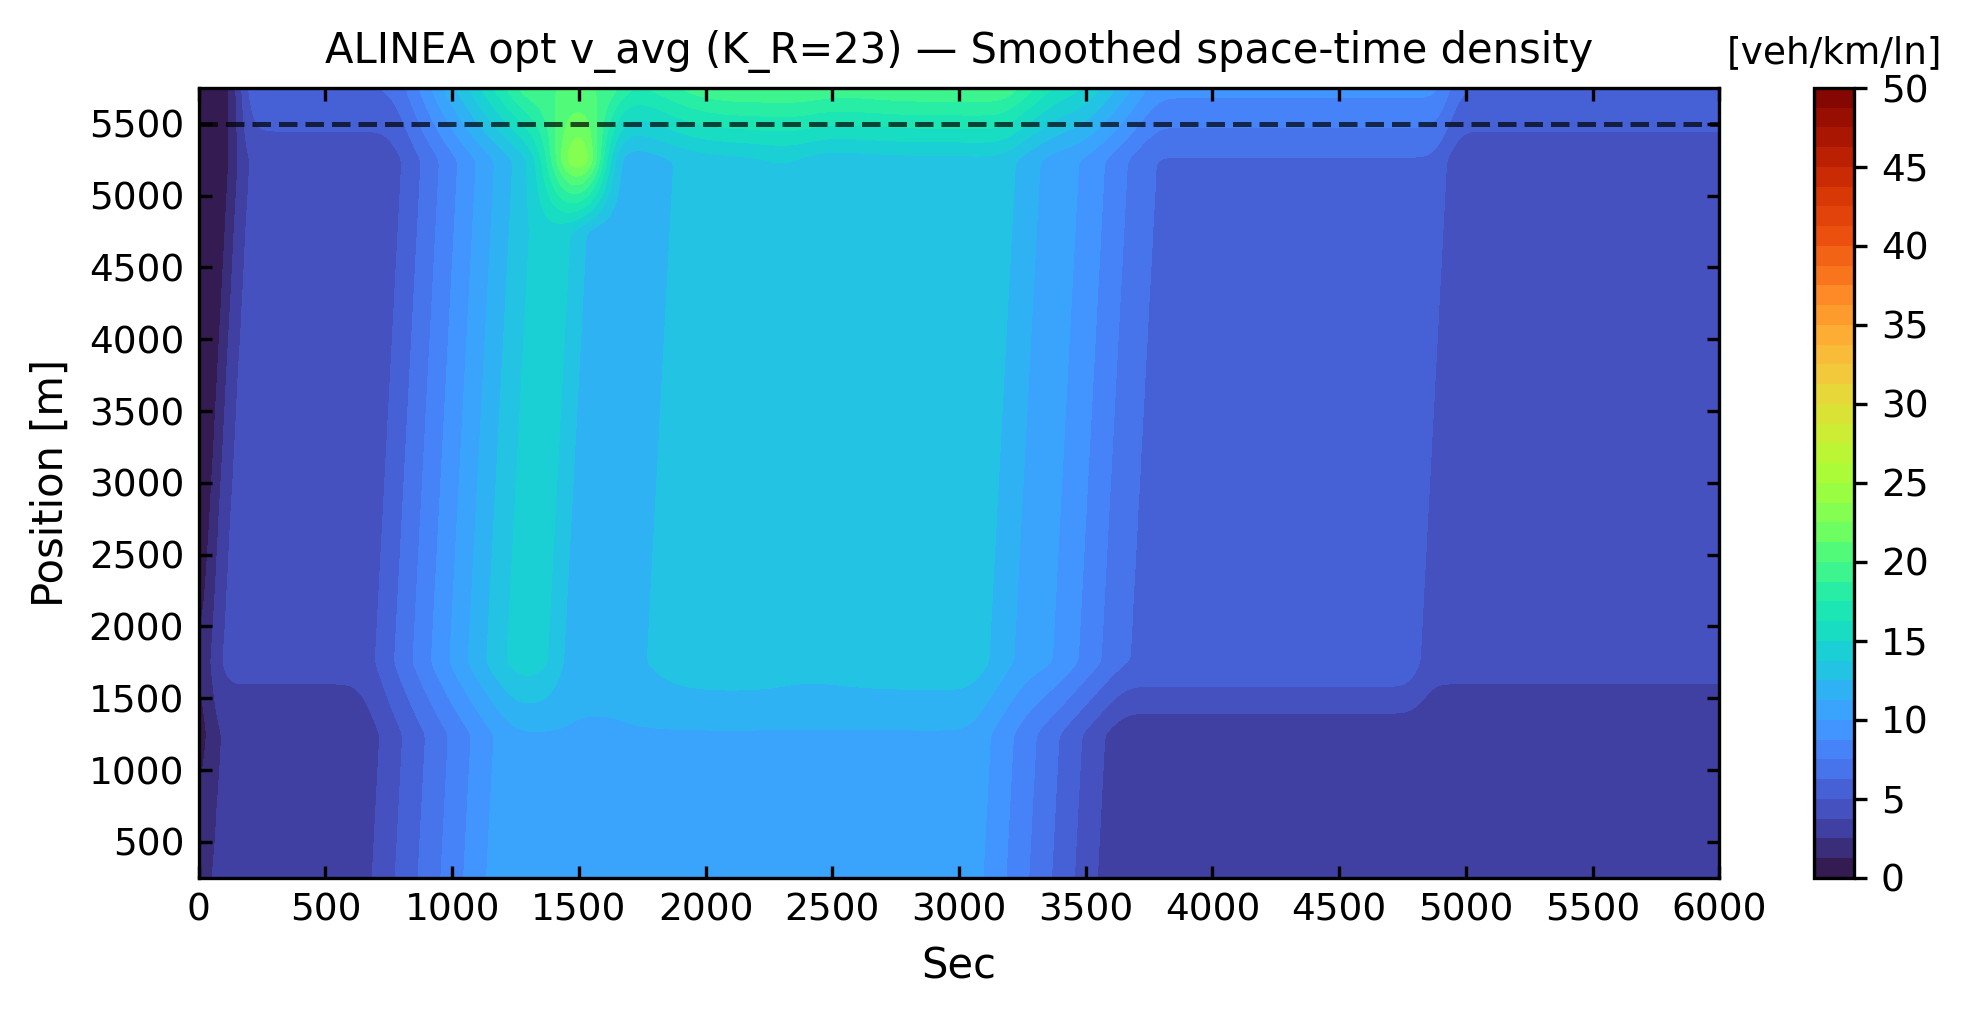
\includegraphics[width=\linewidth]{figures/ALINEA/Opti_no_queue/alinea_opt_vavg_clean_scenario_smoothed.png}
        \caption{ALINEA optimised for
    $\bar{v}$}
        \label{fig:placeholder_opt_spacetime_ali}
    \end{subfigure}
    \hfill
    \begin{subfigure}{0.48\textwidth}
        \centering
        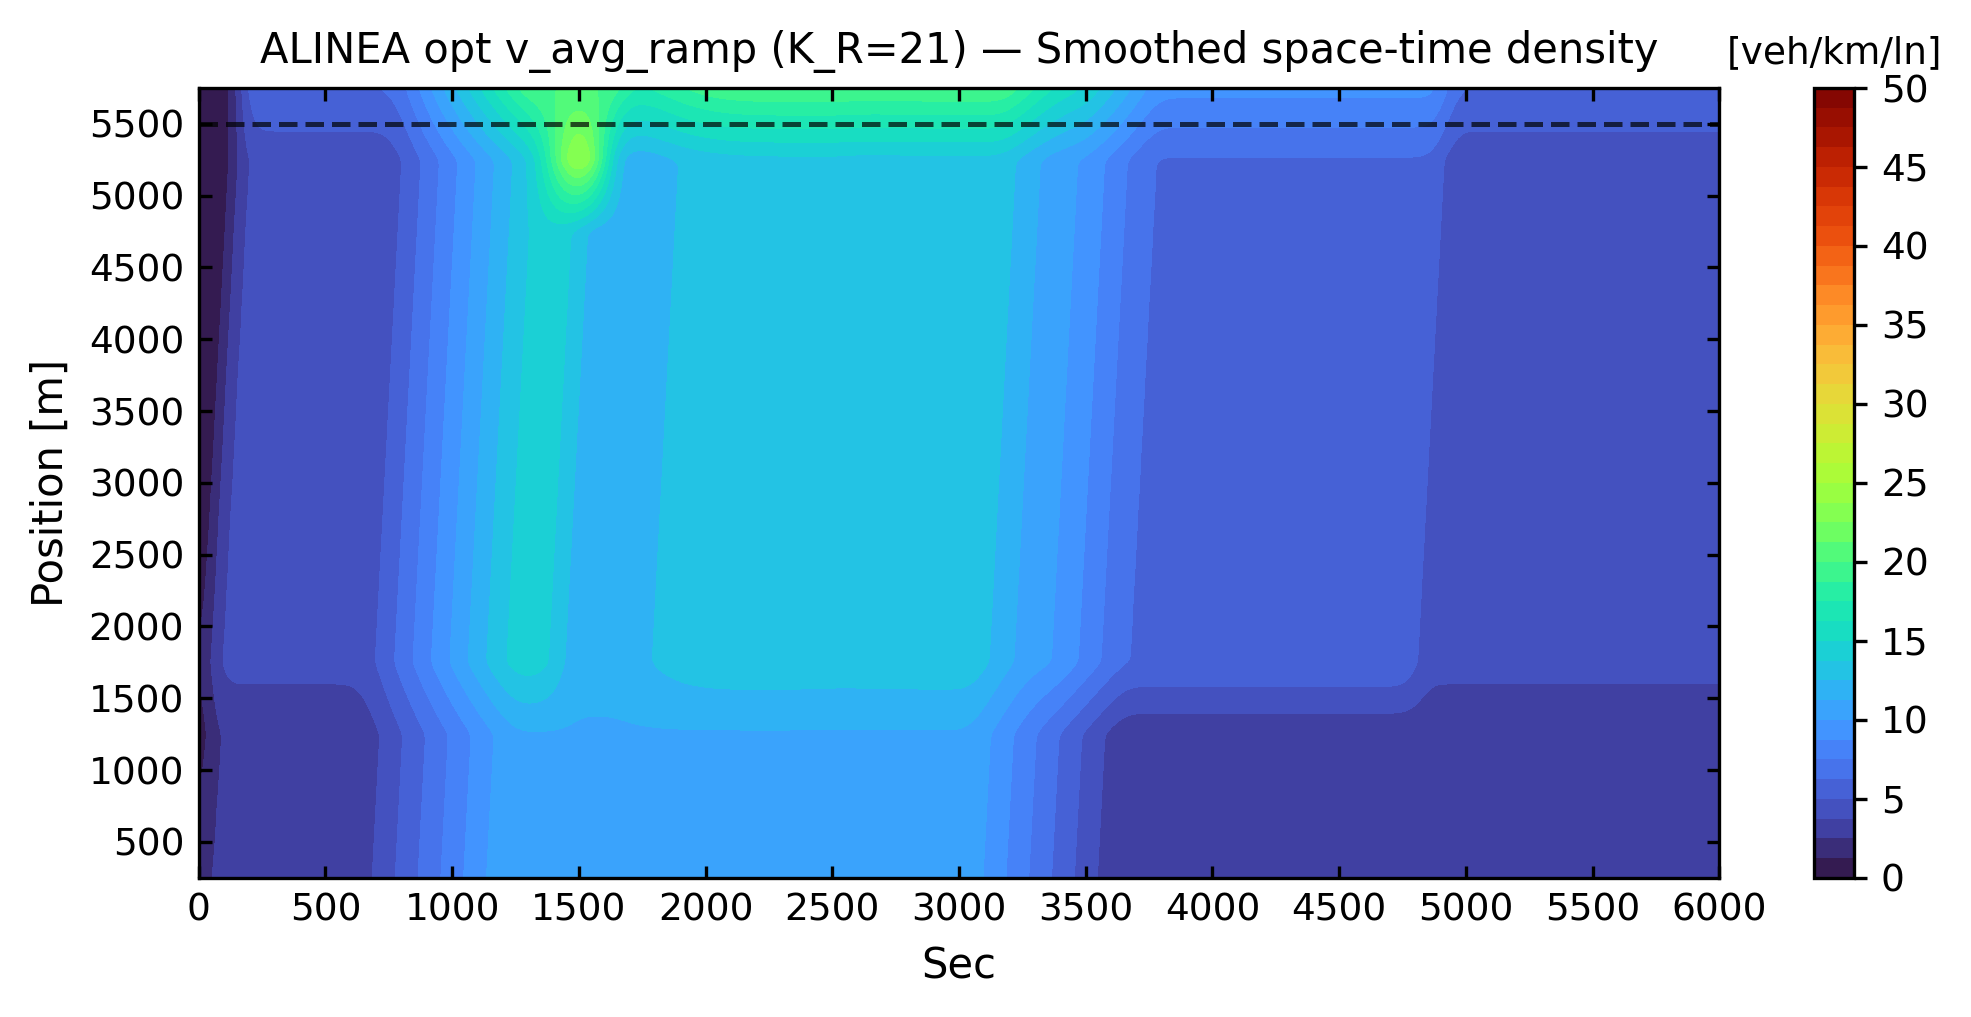
\includegraphics[width=\linewidth]{figures/ALINEA/Opti_with_queue/alinea_opt_vavg_ramp_clean_scenario_smoothed.png}
        \caption{ALINEA optimised for $\bar{v}_\text{queue}$}
        \label{fig:placeholder_opt_spacetime_ali_ramp}
    \end{subfigure}

    \vspace{0.5em}

    \begin{subfigure}{0.48\textwidth}
        \centering
        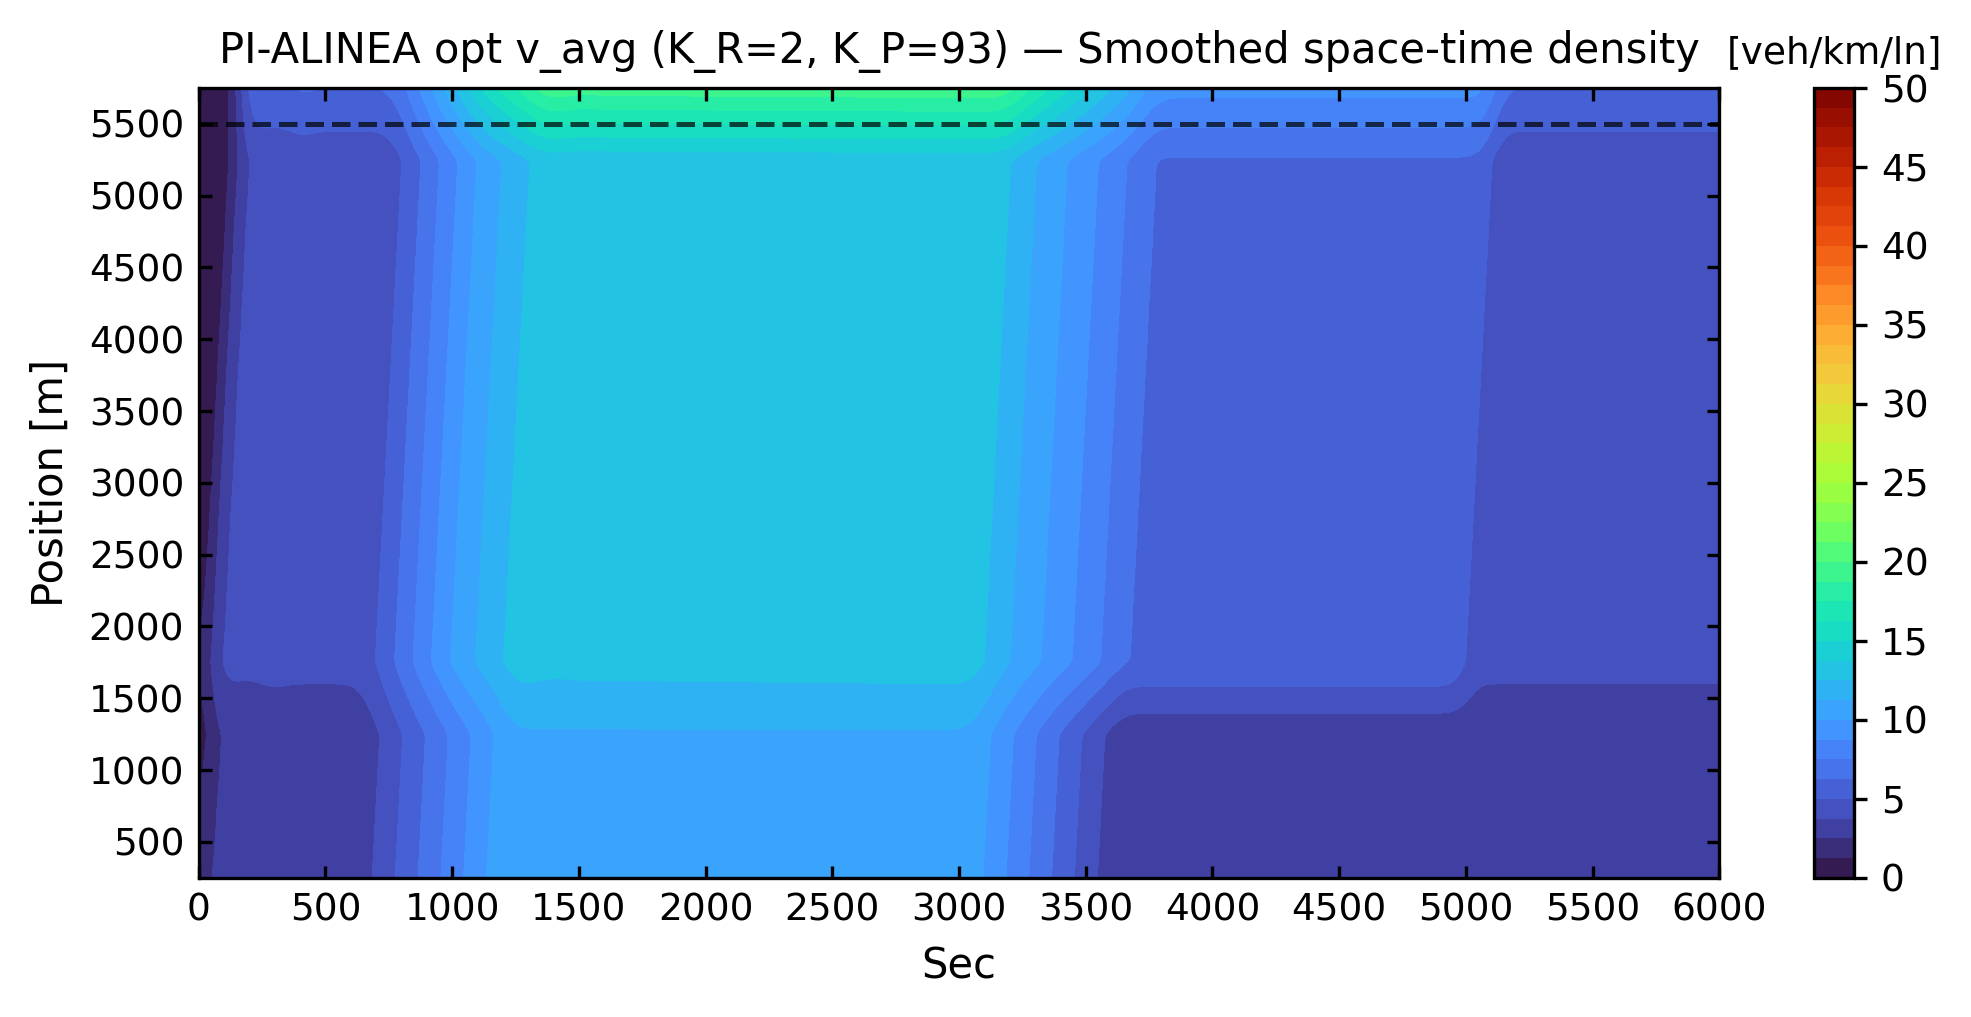
\includegraphics[width=\linewidth]{figures/PI_ALINEA/Opti_no_queue/pi_opt_vavg_clean_scenario_smoothed.png}
        \caption{PI-ALINEA
    optimised for $\bar{v}$}
        \label{fig:placeholder_opt_spacetime_pi}
    \end{subfigure}
    \hfill
    \begin{subfigure}{0.48\textwidth}
        \centering
        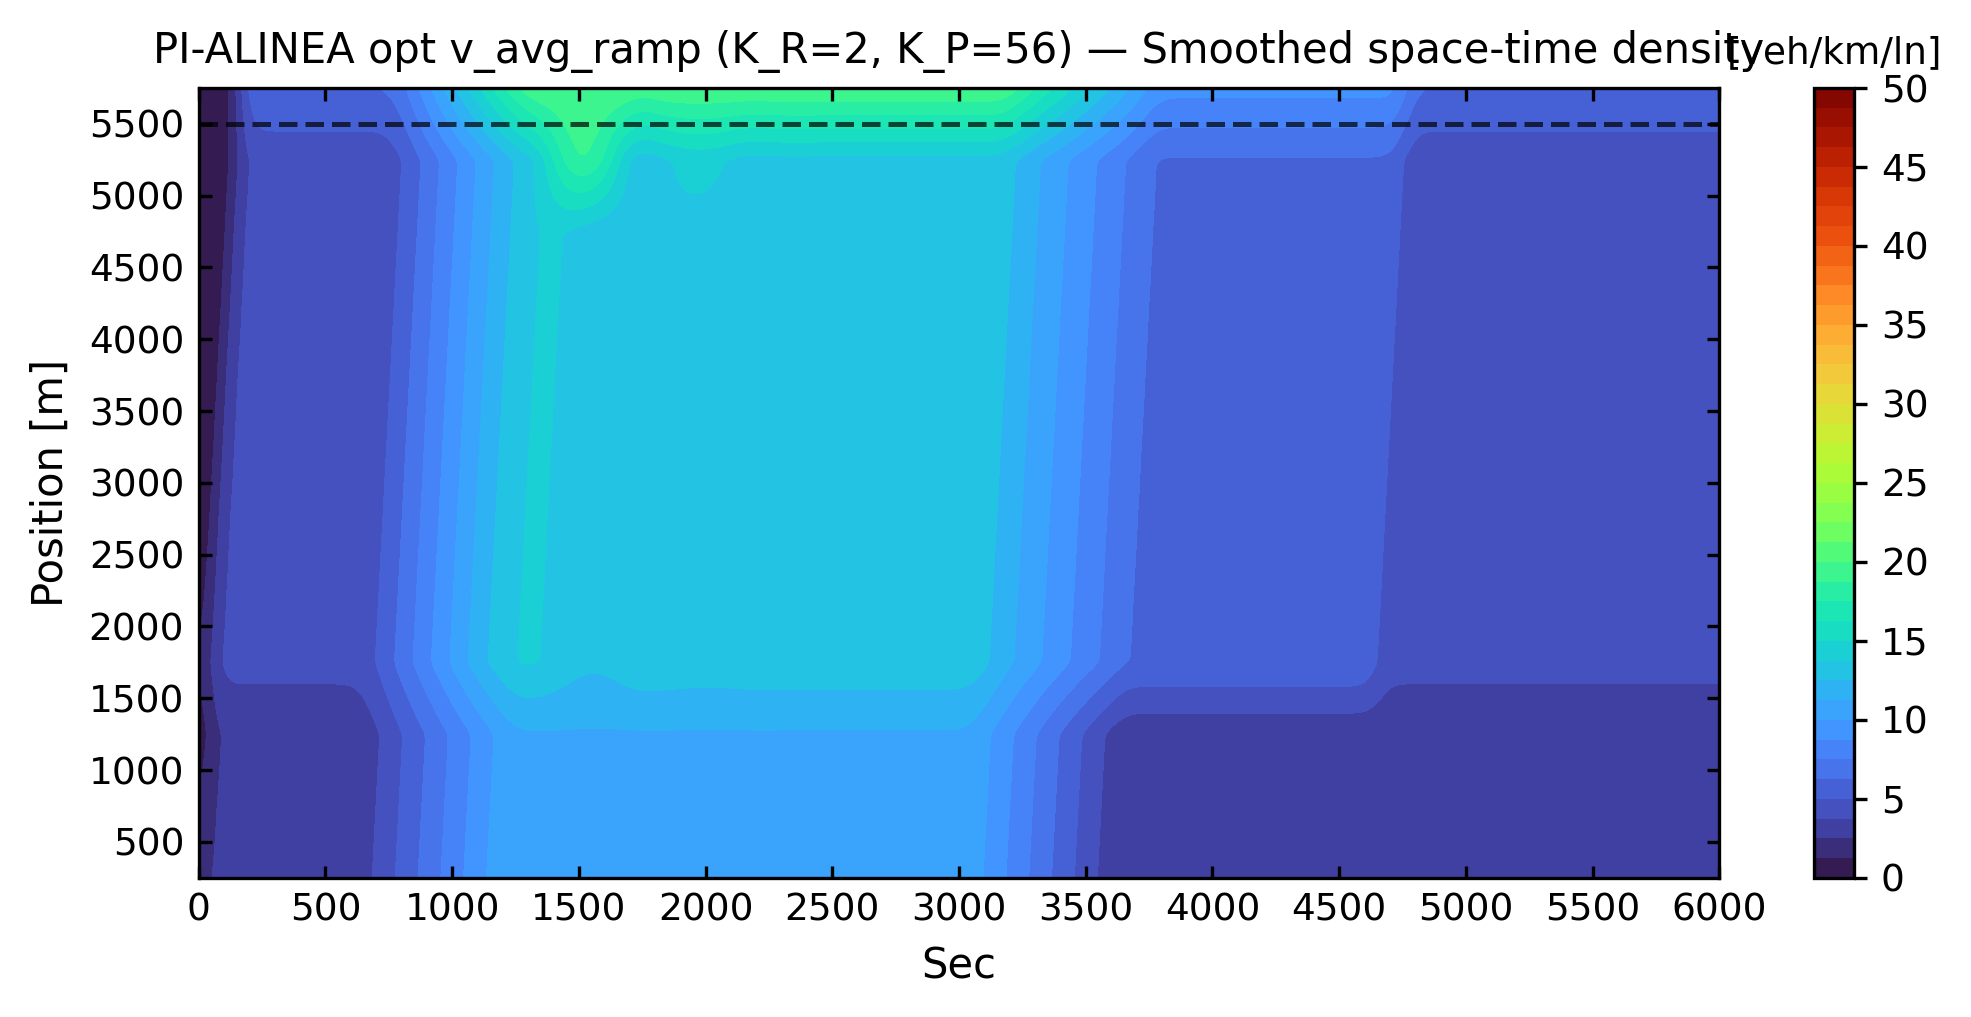
\includegraphics[width=\linewidth]{figures/PI_ALINEA/Opti_with_queue/pi_opt_vavg_ramp_clean_scenario_smoothed.png}
        \caption{PI-ALINEA optimised for
    $\bar{v}_\text{queue}$}
        \label{fig:placeholder_opt_spacetime_pi_ramp}
    \end{subfigure}

    \caption{Optimised benchmark controllers: space--time density contours
    under base demand.}
    \label{fig:placeholder_opt_spacetime}
\end{figure}

\begin{figure}[htbp]
    \centering

    \begin{subfigure}{0.48\textwidth}
        \centering
        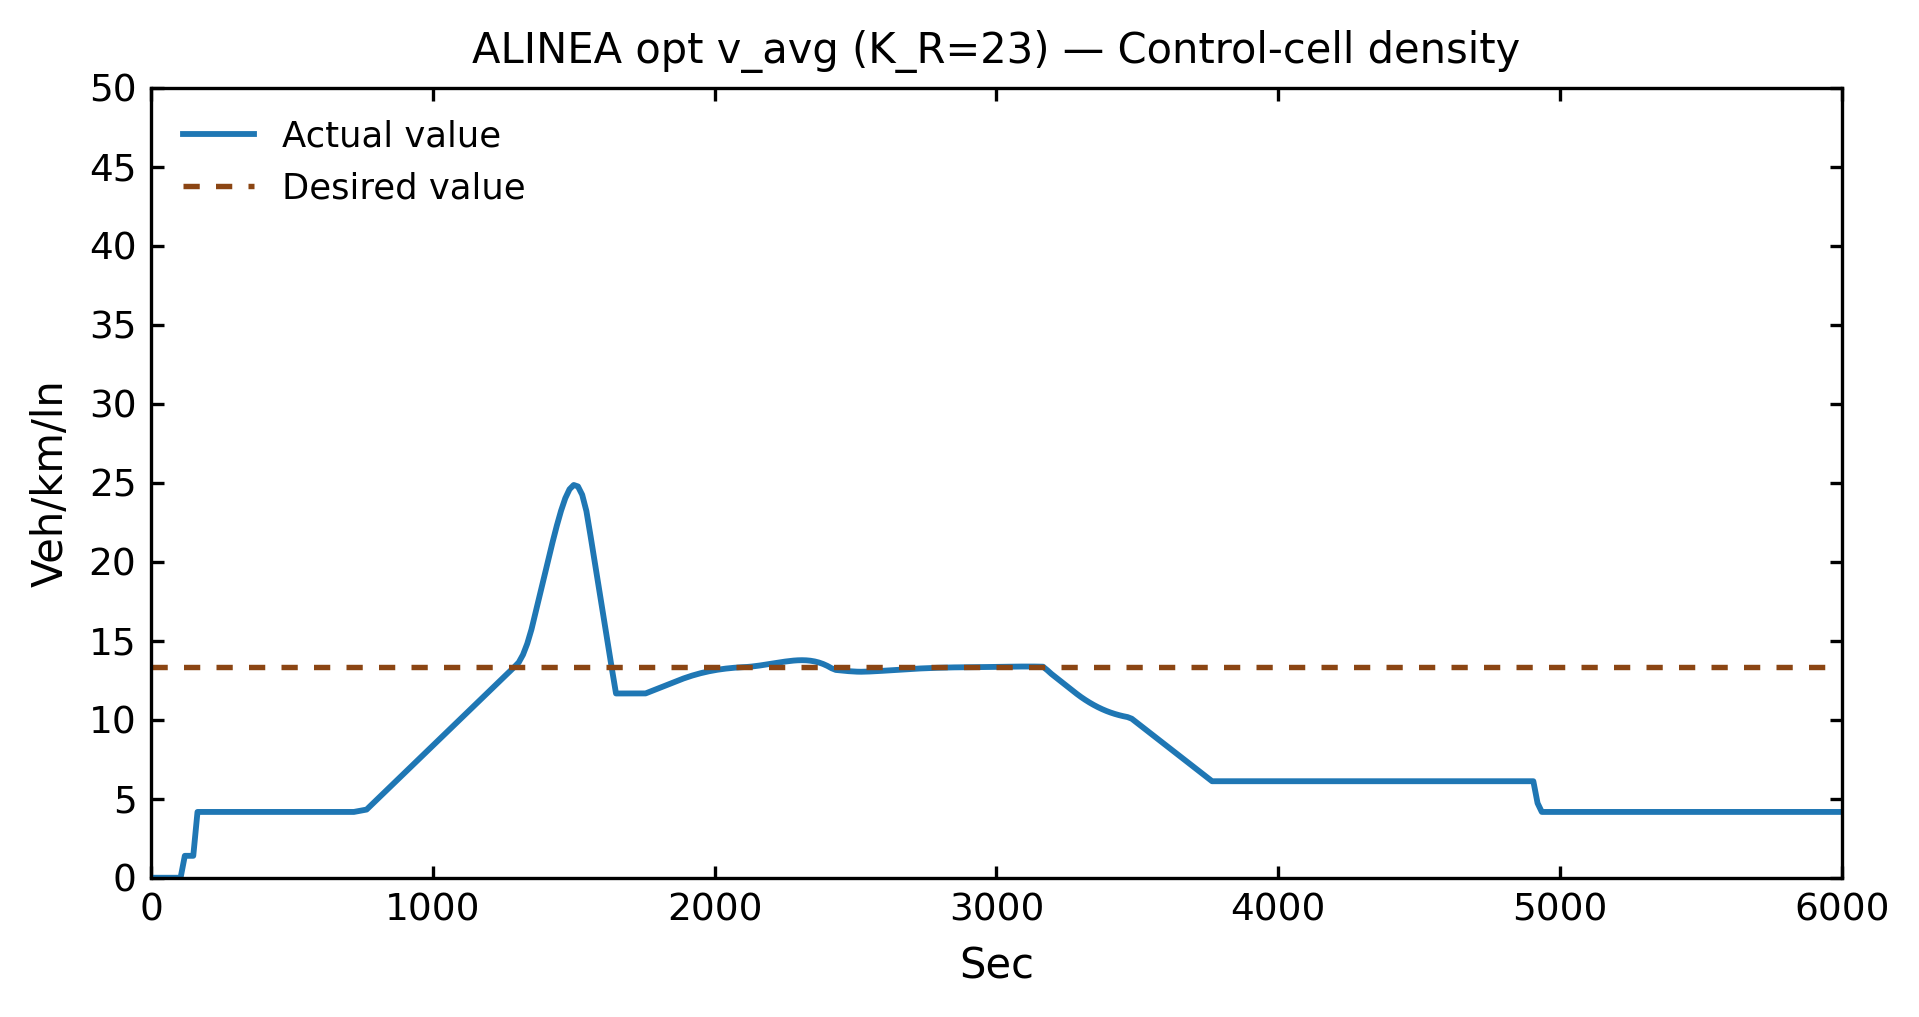
\includegraphics[width=\linewidth]{figures/ALINEA/Opti_no_queue/alinea_opt_vavg_clean_scenario_density.png}
        \caption{ALINEA optimised for
    $\bar{v}$}
        \label{fig:placeholder_opt_control_cell_ali}
    \end{subfigure}
    \hfill
    \begin{subfigure}{0.48\textwidth}
        \centering
        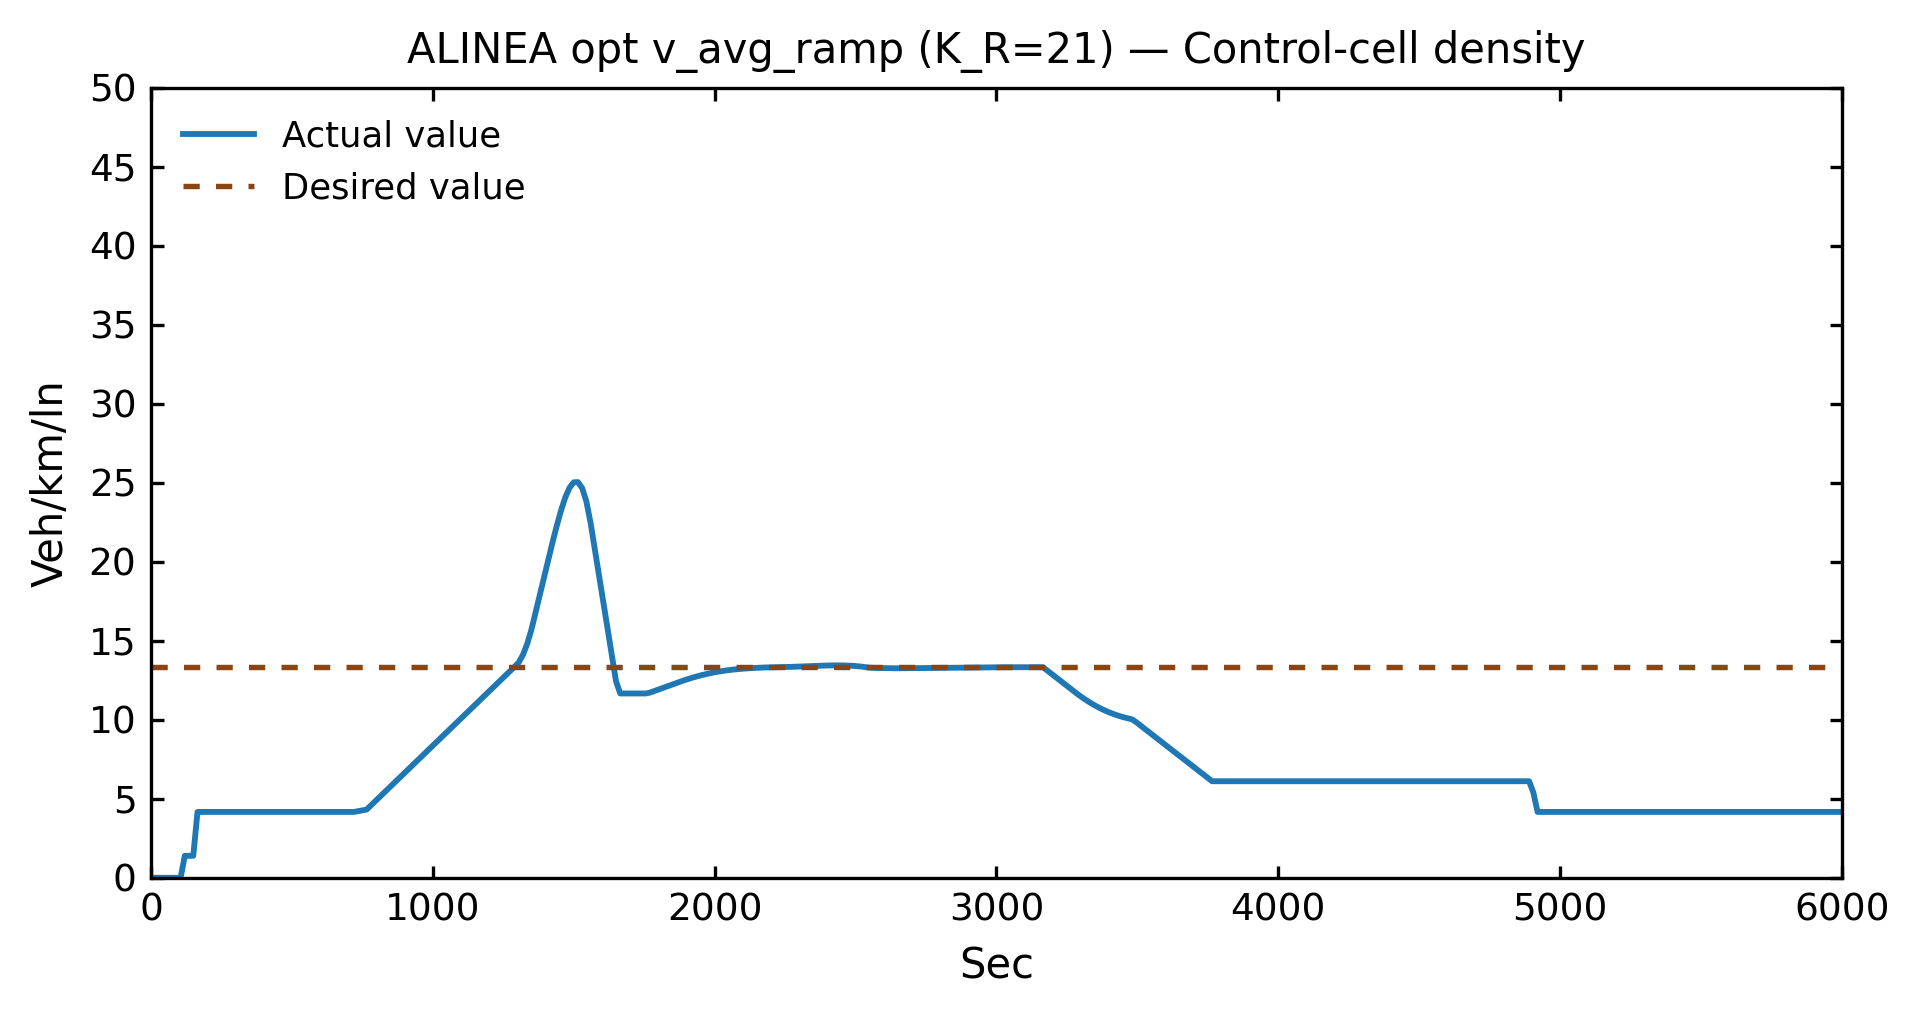
\includegraphics[width=\linewidth]{figures/ALINEA/Opti_with_queue/alinea_opt_vavg_ramp_clean_scenario_density.png}
        \caption{ALINEA optimised for $\bar{v}_\text{queue}$}
        \label{fig:placeholder_opt_control_cell_ali_ramp}
    \end{subfigure}

    \vspace{0.5em}

    \begin{subfigure}{0.48\textwidth}
        \centering
        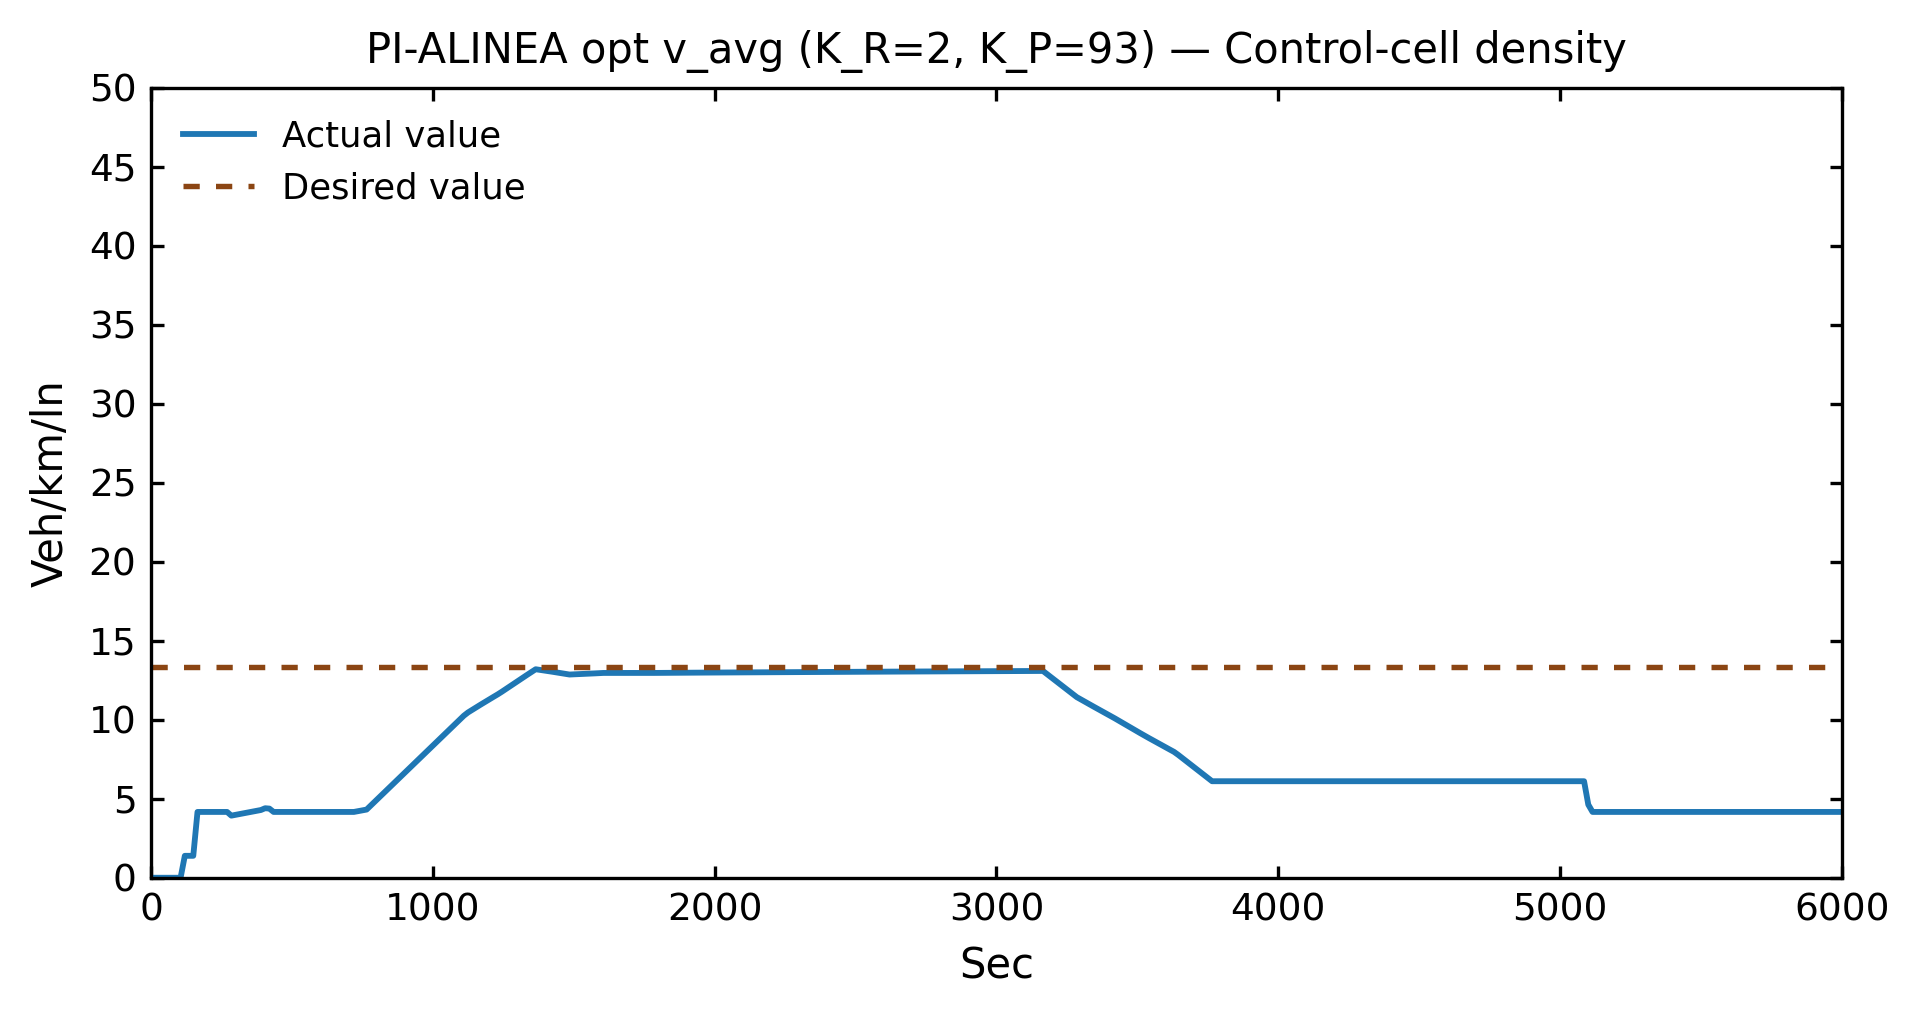
\includegraphics[width=\linewidth]{figures/PI_ALINEA/Opti_no_queue/pi_opt_vavg_clean_scenario_density.png}
        \caption{PI-ALINEA
    optimised for $\bar{v}$}
        \label{fig:placeholder_opt_control_cell_pi}
    \end{subfigure}
    \hfill
    \begin{subfigure}{0.48\textwidth}
        \centering
        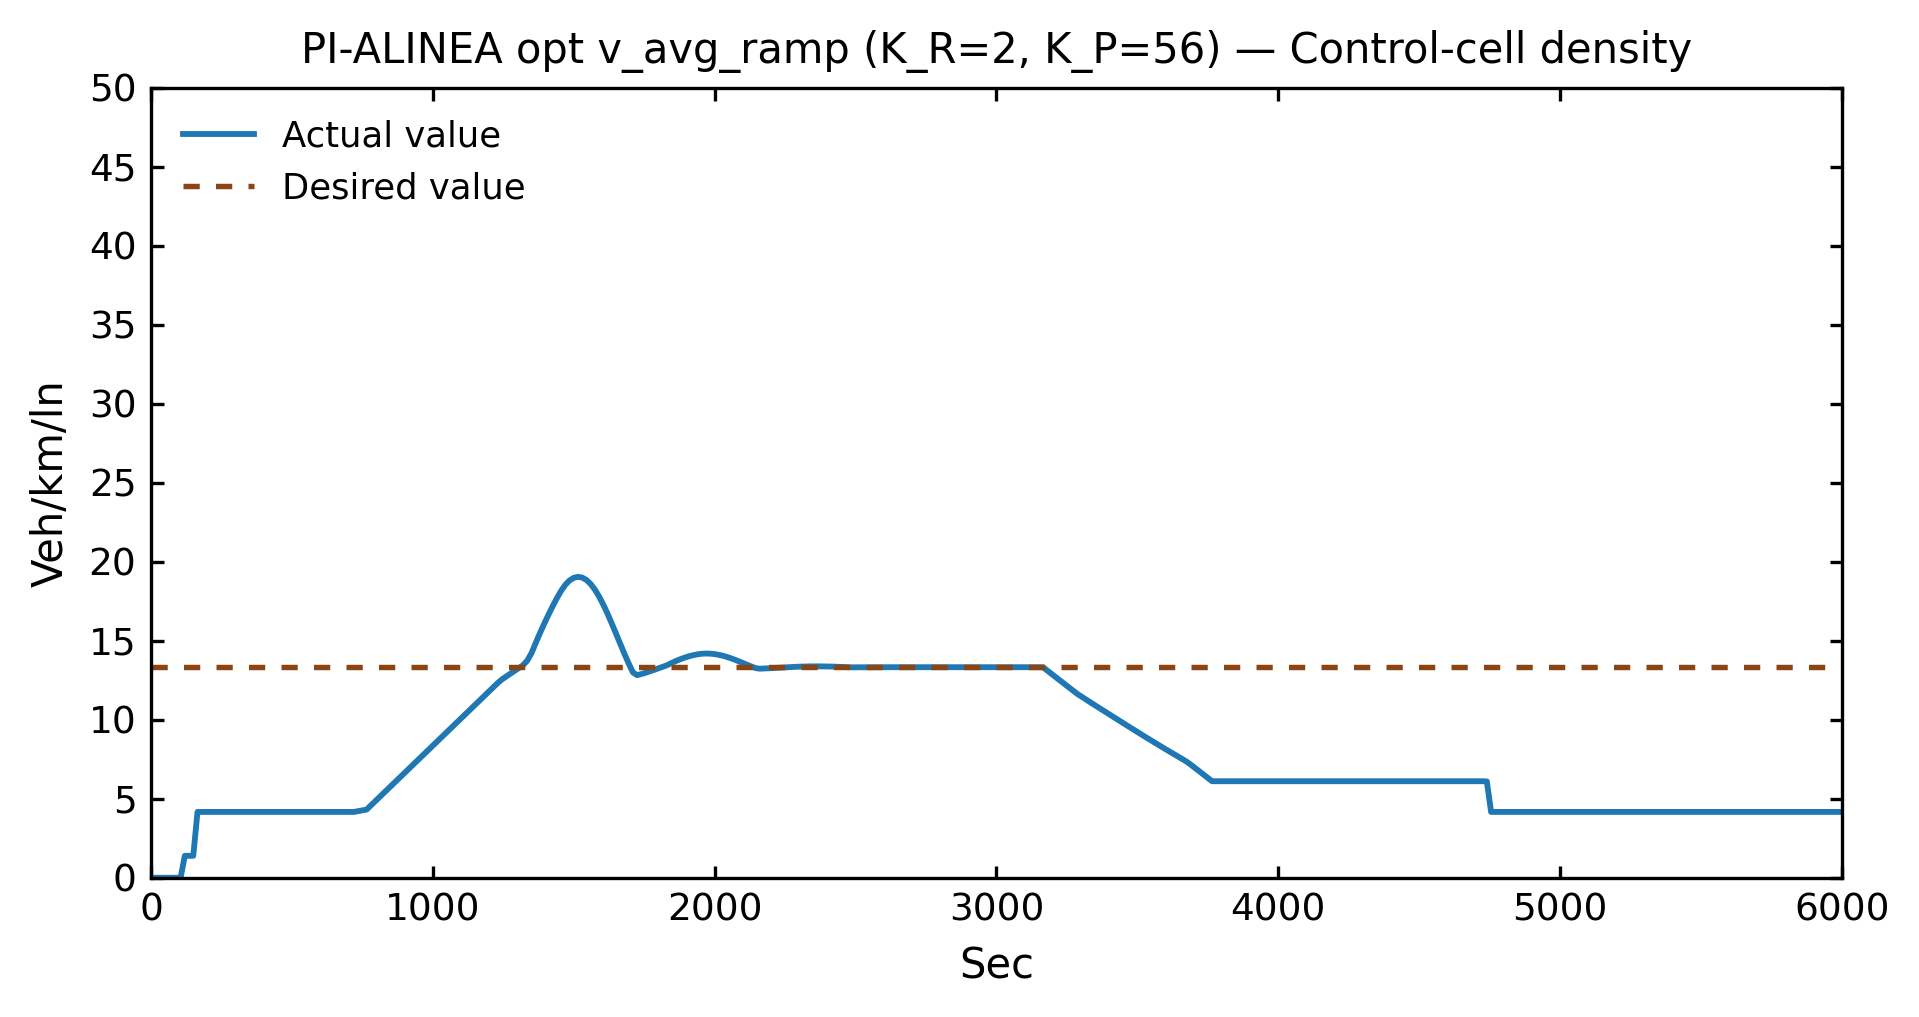
\includegraphics[width=\linewidth]{figures/PI_ALINEA/Opti_with_queue/pi_opt_vavg_ramp_clean_scenario_density.png}
        \caption{PI-ALINEA optimised for
    $\bar{v}_\text{queue}$}
        \label{fig:placeholder_opt_control_cell_pi_ramp}
    \end{subfigure}

    \caption{Optimised benchmark controllers: control-cell density under base demand.}
    \label{fig:placeholder_opt_control_cell}
\end{figure}

\begin{figure}[htbp]
    \centering

    \begin{subfigure}{0.48\textwidth}
        \centering
        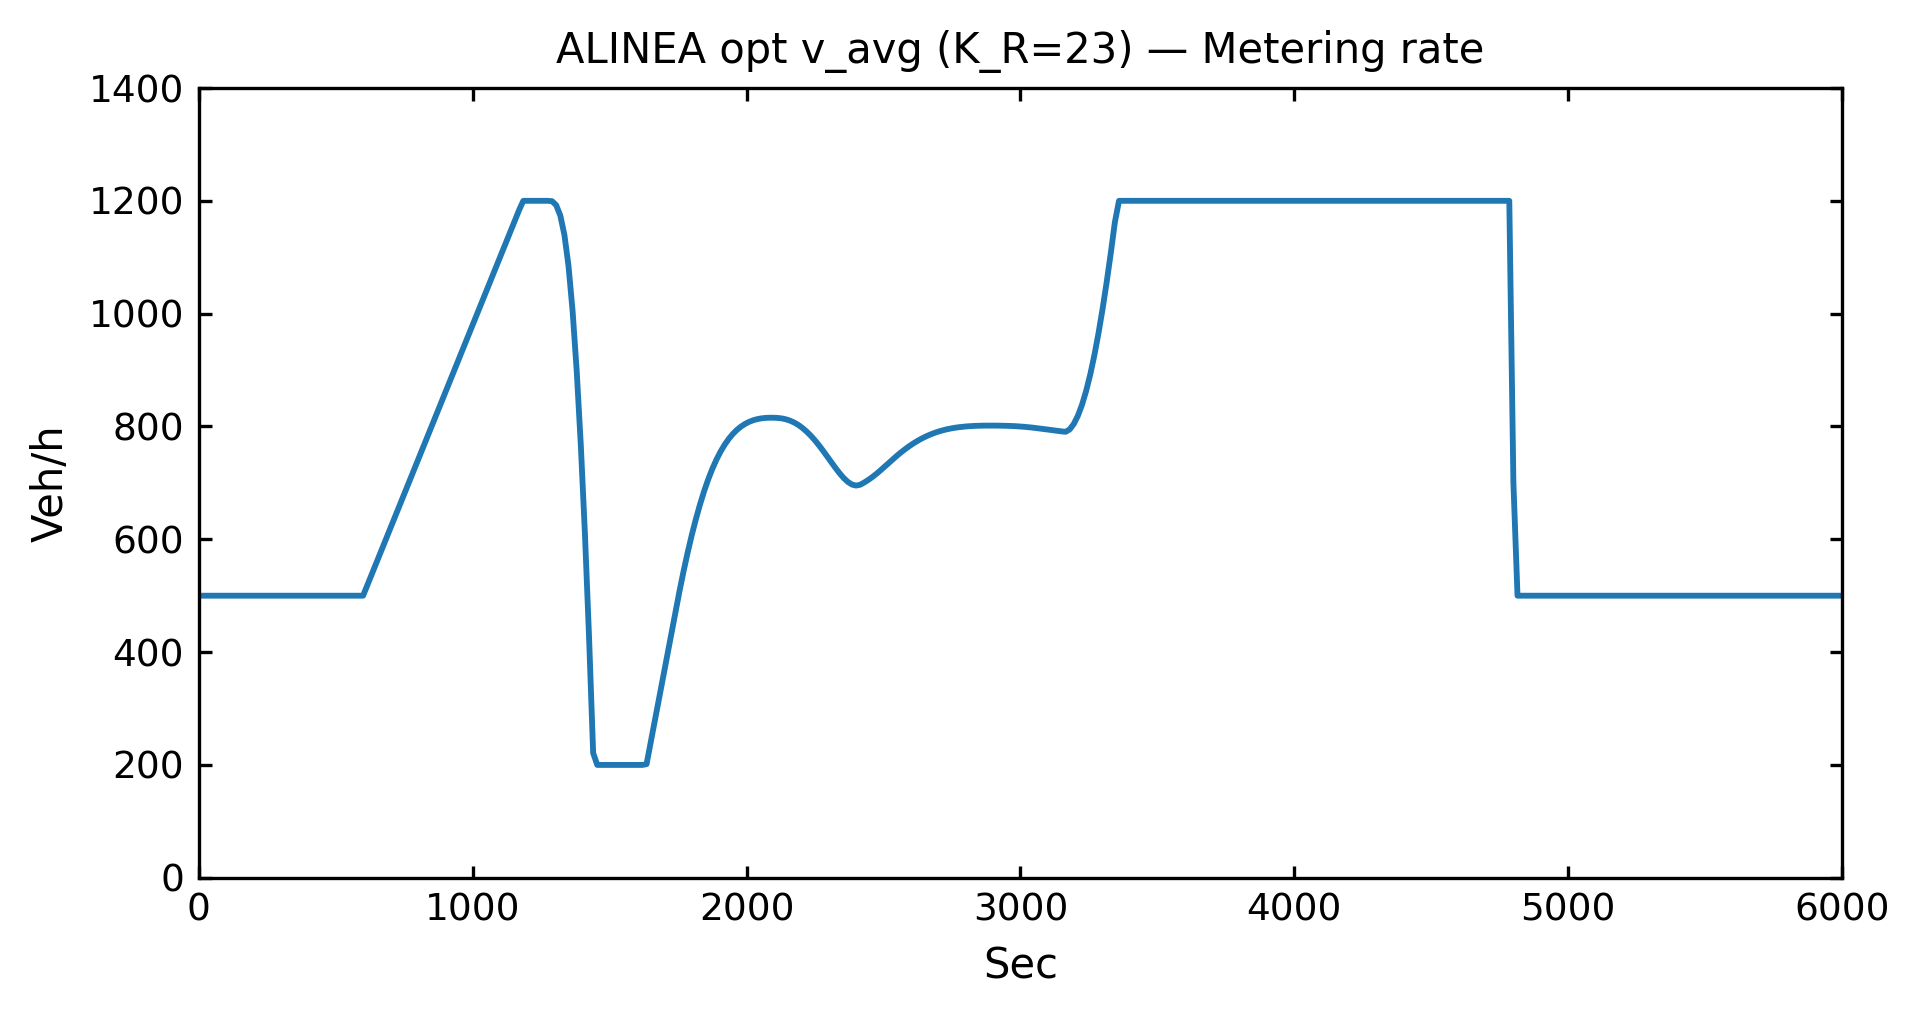
\includegraphics[width=\linewidth]{figures/ALINEA/Opti_no_queue/alinea_opt_vavg_clean_metering_rate.png}
        \caption{ALINEA optimised for
    $\bar{v}$}
        \label{fig:placeholder_opt_metering_ali}
    \end{subfigure}
    \hfill
    \begin{subfigure}{0.48\textwidth}
        \centering
        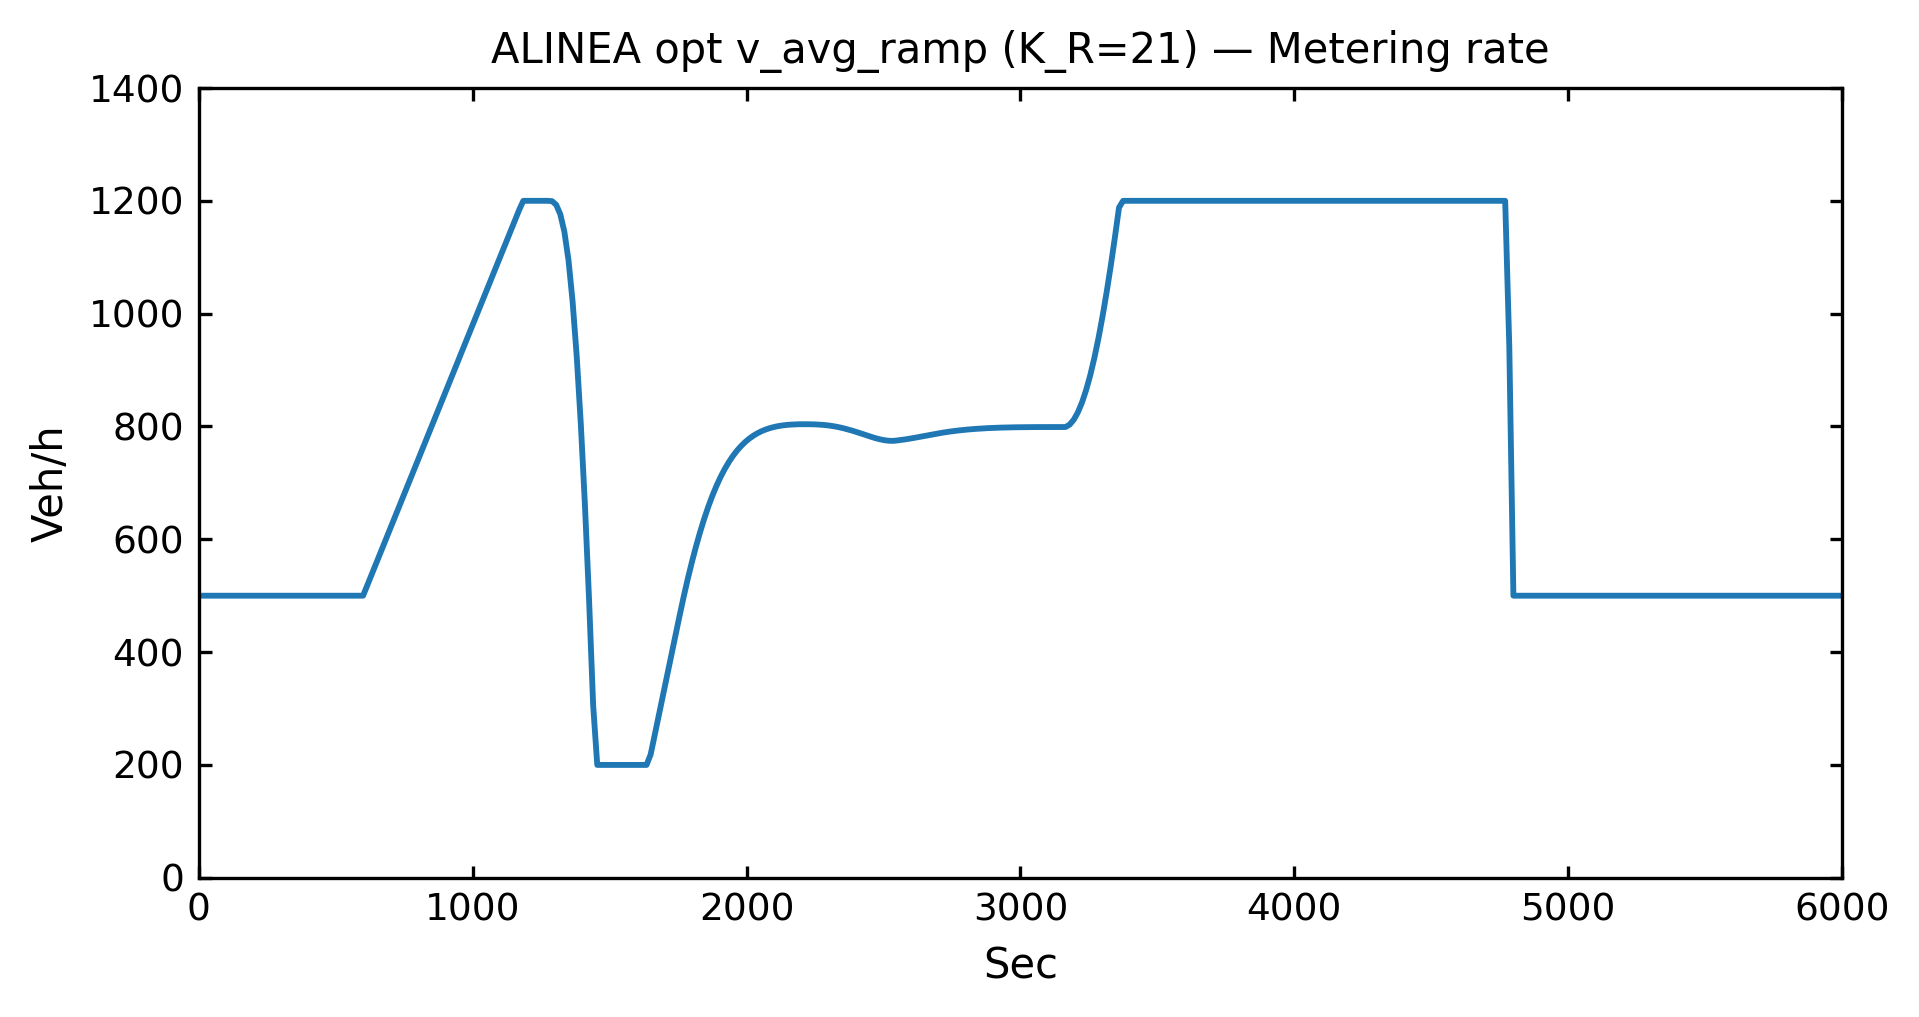
\includegraphics[width=\linewidth]{figures/ALINEA/Opti_with_queue/alinea_opt_vavg_ramp_clean_metering_rate.png}
        \caption{ALINEA optimised for $\bar{v}_\text{queue}$}
        \label{fig:placeholder_opt_metering_ali_ramp}
    \end{subfigure}

    \vspace{0.5em}

    \begin{subfigure}{0.48\textwidth}
        \centering
        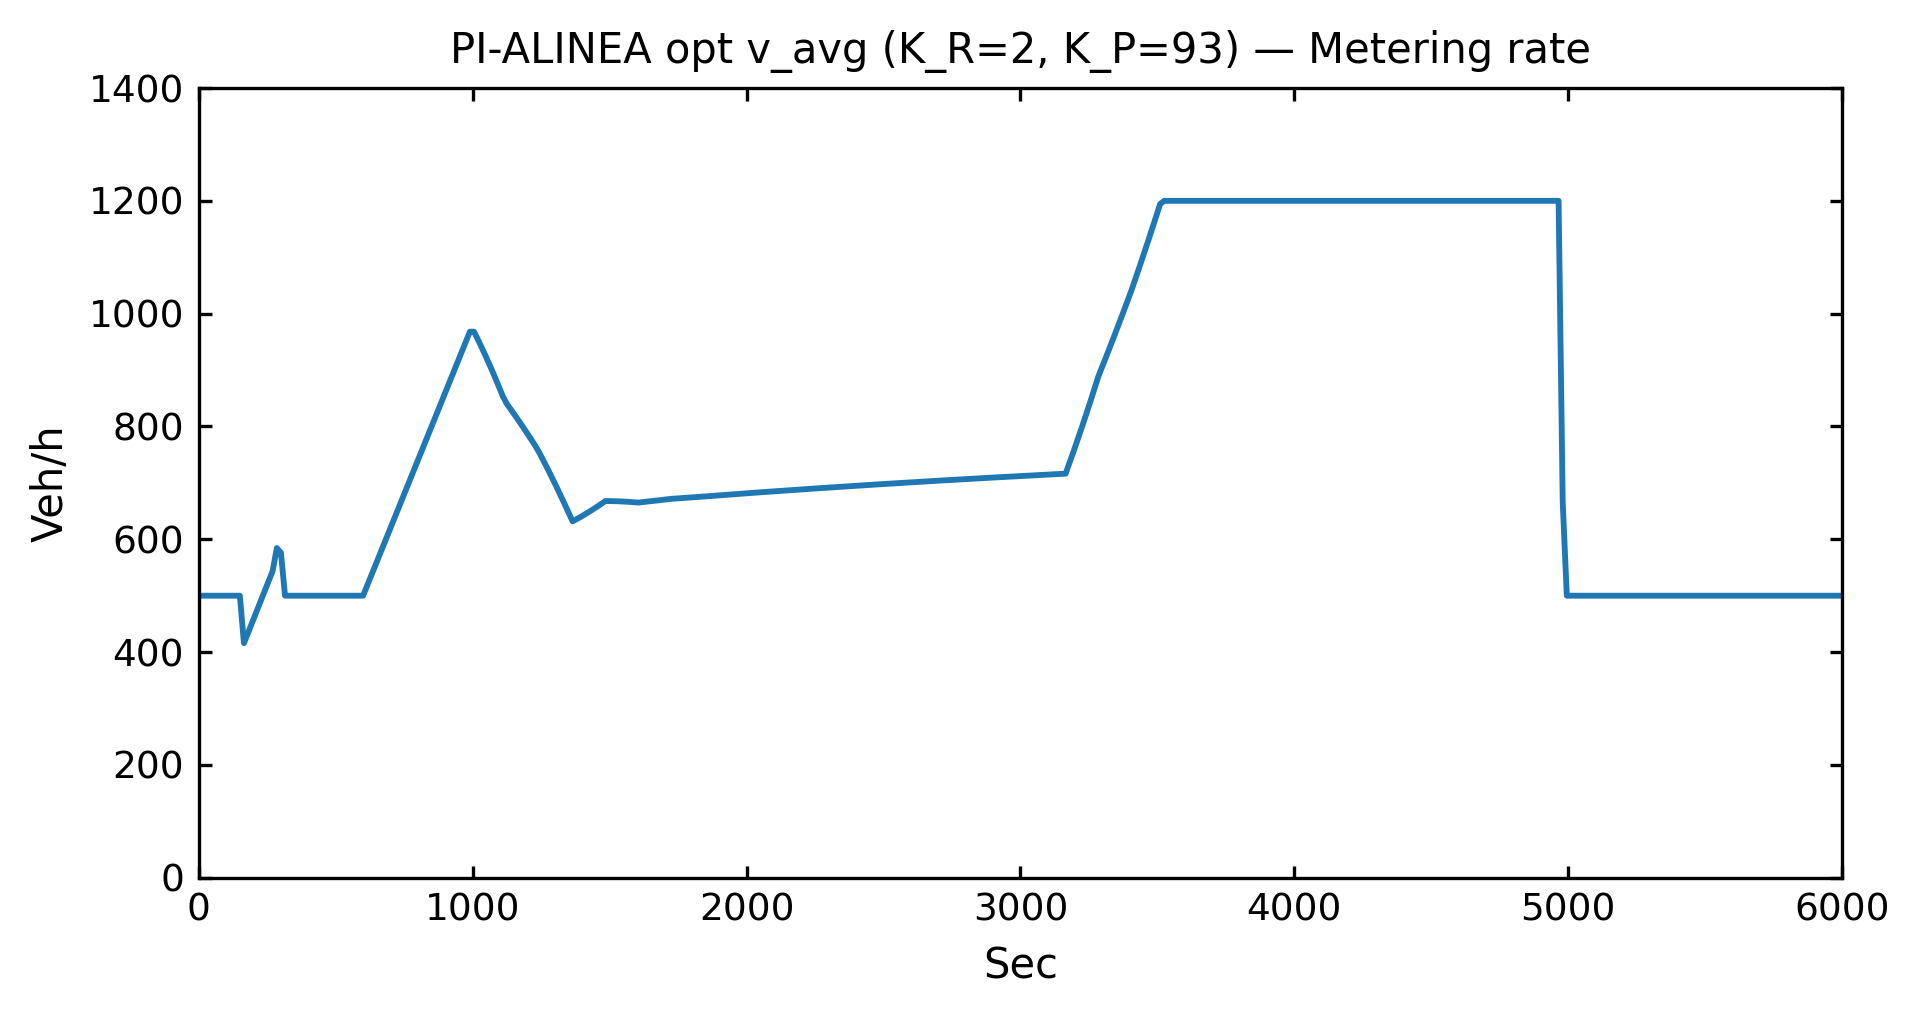
\includegraphics[width=\linewidth]{figures/PI_ALINEA/Opti_no_queue/pi_opt_vavg_clean_metering_rate.png}
        \caption{PI-ALINEA
    optimised for $\bar{v}$}
        \label{fig:placeholder_opt_metering_pi}
    \end{subfigure}
    \hfill
    \begin{subfigure}{0.48\textwidth}
        \centering
        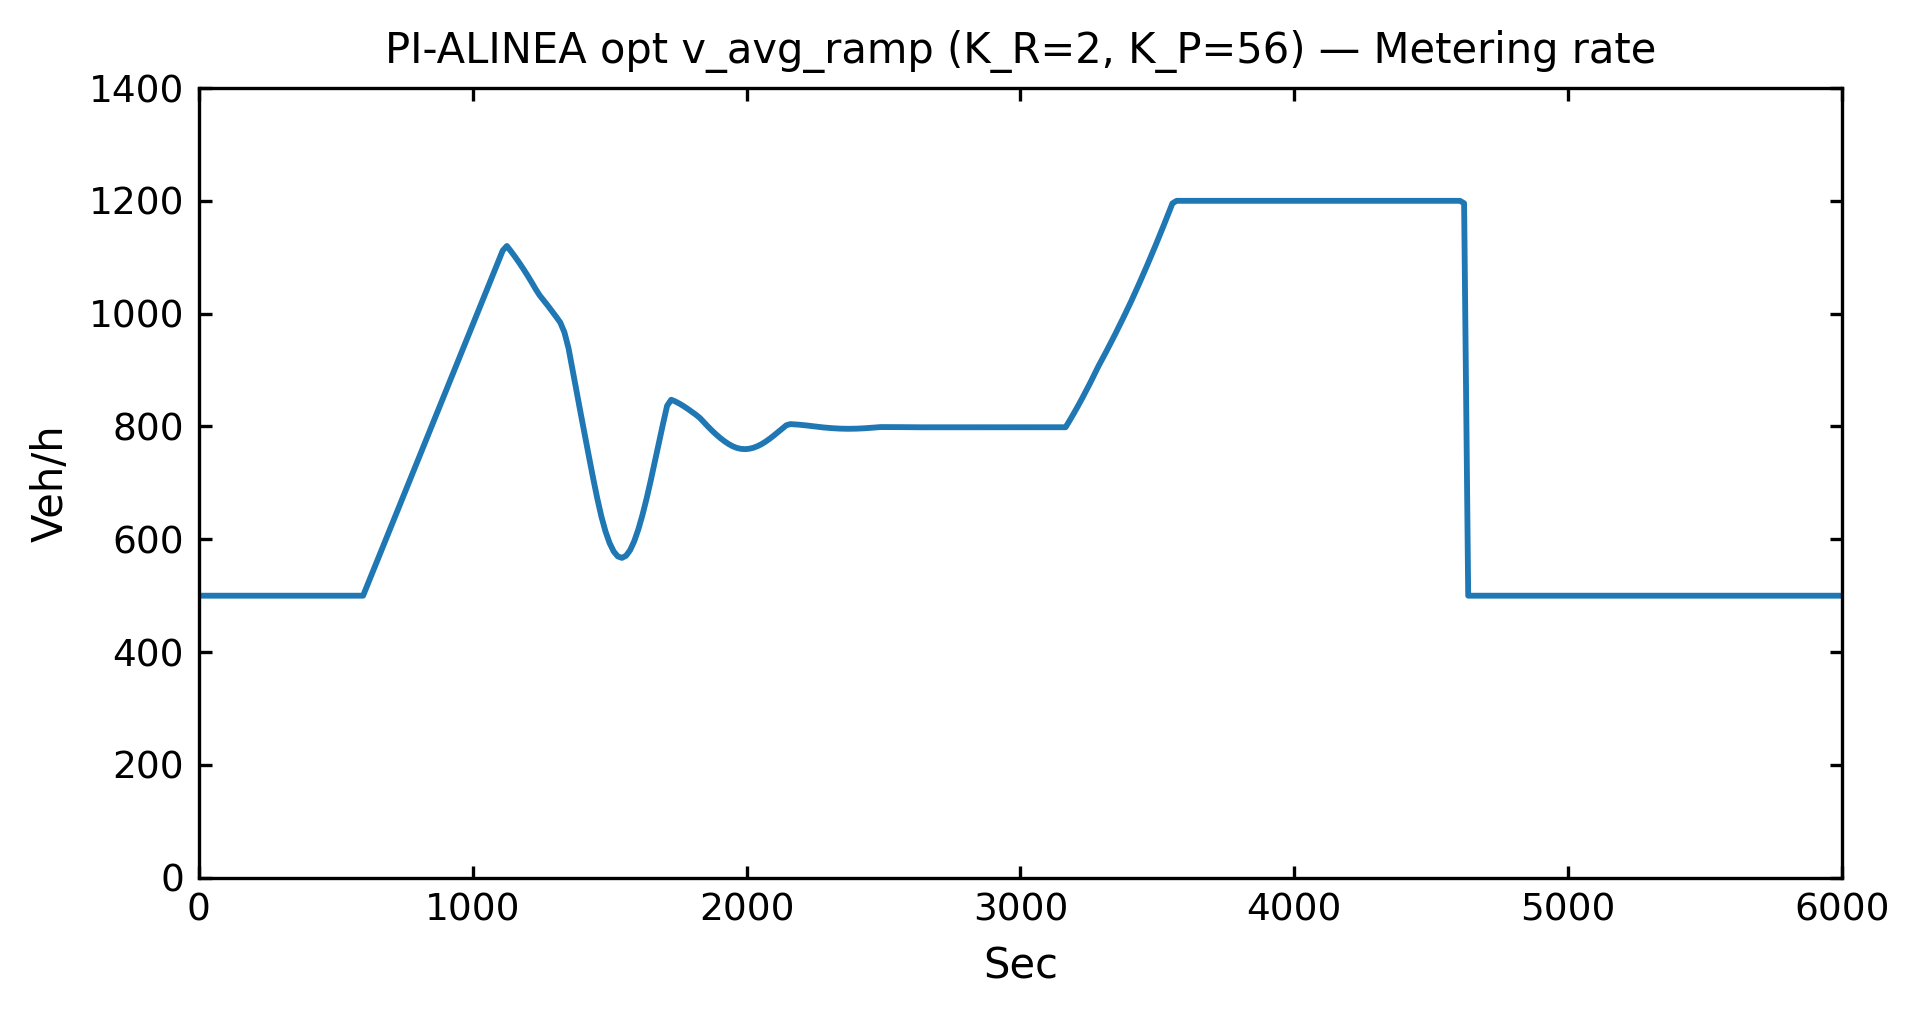
\includegraphics[width=\linewidth]{figures/PI_ALINEA/Opti_with_queue/pi_opt_vavg_ramp_clean_metering_rate.png}
        \caption{PI-ALINEA optimised for
    $\bar{v}_\text{queue}$}
        \label{fig:placeholder_opt_metering_pi_ramp}
    \end{subfigure}

    \caption{Optimised benchmark controllers: on-ramp entry rate under base demand.}
    \label{fig:placeholder_opt_metering}
\end{figure}

The control-cell density trajectories in
Figure~\ref{fig:placeholder_opt_control_cell} further indicate that the optimised
PI-ALINEA controllers are more effective at maintaining the density close to the
desired value. In particular, the PI-ALINEA controller optimised for
\(\bar{v}\) appears to keep the control-cell density closest to
\(\rho_{\mathrm{des}}\), suggesting that optimizing this controller to maximise the mainline average speed
also partly coincides with maximizing the density-based reward used by the RL agent.
This is consistent with the definition of the reward function, which directly
penalises deviations of the control-cell density from the desired density.

The space--time density contours in
Figure~\ref{fig:placeholder_opt_spacetime} support the same interpretation. The
optimised controllers limit the formation of high-density regions near the
lane-drop and produce smoother traffic patterns than the reference PI-ALINEA
configuration. The queue-aware optimisation criterion
\(\bar{v}_{\mathrm{queue}}\) leads to slightly more conservative control
settings, as expected, because the objective also penalises ramp waiting time.
Quantitative performance of all controllers across all demand scenarios is reported in
Table~\ref{tab:full_results}. 


\subsection{RL Agent}\label{subsec:RL}

\subsubsection{Training Behaviour}

A total of six independent RL training campaigns were conducted. Four campaigns
used an \(\epsilon\)-greedy exploration policy with a lower exploration bound of
\(\epsilon_{\min}=0.05\), while two campaigns allowed \(\epsilon\) to decay
without a lower bound. Since the original article does not specify the
\(\epsilon\)-decay schedule or the convergence criterion used during training,
all campaigns were run up to the reported training length of 700,000 episodes.

Figure~\ref{fig:rl_training_curves} shows representative training curves for
one capped and one uncapped exploration campaign. The remaining campaigns
showed similar qualitative behaviour. In general, the training process did not converge towards a stable final policy. Instead,
policy quality varied across checkpoints, with the final networks at
700,000 episodes not necessarily being the best-performing policy.

Both the learning curve and the 1000-episode rolling reward standard deviation show that the capped exploration policy reaches a plateau
after approximately \(200{,}000\)--\(300{,}000\) episodes. Beyond this point,
the rolling mean remains within a relatively stable reward interval, which is
consistent with the exploration probability reaching its lower bound of
\(\epsilon_{\min}=0.05\). Continued exploration therefore prevents the policy
from becoming fully deterministic and maintains persistent variability in the
episode rewards.

In the uncapped case, the reward variance decreases more strongly as
\(\epsilon\) approaches zero, indicating a transition towards an increasingly
deterministic policy. However, the absence of continued exploration also makes
the training process more sensitive to occasional poor updates. Once the policy
has become nearly deterministic, such updates can lead to a degradation of the
learned behaviour from which recovery is difficult. This behaviour is visible
in the later part of the uncapped learning curve (see Figure \ref{fig:rl_training_curves}). 

\begin{figure}[htbp]
    \centering

    \begin{subfigure}{0.48\textwidth}
        \centering
        
\includegraphics[width=\linewidth]{figures/RL/learning/epsilon_5/06_07_learning_curve.png}
        \caption{Learning curve, $\epsilon_{\min}=0.05$}
    \end{subfigure}
    \hfill
    \begin{subfigure}{0.48\textwidth}
        \centering
        
\includegraphics[width=\linewidth]{figures/RL/learning/epsilon_0/06_07_learning_curve.png}
        \caption{Learning curve, no exploration floor}
    \end{subfigure}

    \vspace{0.6em}

    \begin{subfigure}{0.48\textwidth}
        \centering
        
\includegraphics[width=\linewidth]{figures/RL/learning/epsilon_5/06_07_reward_rolling_std.png}
        \caption{Rolling reward standard deviation, $\epsilon_{\min}=0.05$}
    \end{subfigure}
    \hfill
    \begin{subfigure}{0.48\textwidth}
        \centering
        
\includegraphics[width=\linewidth]{figures/RL/learning/epsilon_0/06_07_reward_rolling_std.png}
        \caption{Rolling reward standard deviation, no exploration floor}
    \end{subfigure}

    \caption{Representative RL training behaviour for exploration with and
    without a lower exploration bound. The top row shows the episode reward and
    rolling mean, while the bottom row shows the rolling standard deviation of
    the training reward.}
    \label{fig:rl_training_curves}
\end{figure}

While no convergence towards an optimal solution could clearly be observed with either exploration scheme, it was noted that the six training runs all reached the same best observed training episode reward of
\(-2049.5\) (see Figure \ref{fig:rl_training_curves}). This suggests that the corresponding episode may represent a
near-optimal metering trajectory for the reconstructed demand scenario.
However, since this reward was obtained during \(\epsilon\)-greedy training, it
does not imply that the ANN learned a deterministic policy capable of
reproducing this trajectory.

\subsubsection{Checkpoint Selection}

The observations above motivated an additional checkpoint-selection procedure.
Since the final checkpoint was not necessarily the best-performing policy, and
since the best training episode may partly depend on exploratory actions, both
exploration variants were rerun with deterministic greedy evaluation performed
after every episode. In this evaluation step, the ANN selected only the action
with the highest predicted value, without \(\epsilon\)-greedy exploration. This
procedure was not specified in the original study.

In these additional runs, both exploration variants reached the same best greedy
episode reward of \(-2062.83\). The corresponding ANN checkpoint was selected
from one of these equivalent best-performing policies for the final comparison.
This reward remained below the best exploratory training reward of \(-2049.5\),
indicating that the best metering trajectory encountered during training was not
recovered by the ANN as a deterministic greedy policy.



\subsubsection{Performance of the selected RL Policy}

The most performant RL policy was then evaluated under the same base demand
scenario used for the benchmark controllers. Figures
\ref{fig:rl_spacetime}, ~\ref{fig:rl_control_cell} and~\ref{fig:rl_metering} show the resulting
control-cell density, on-ramp metering rate, and space--time density contour.
These figures are compared against the corresponding results reported in the
original study.

\begin{figure}[ht]
    \centering
    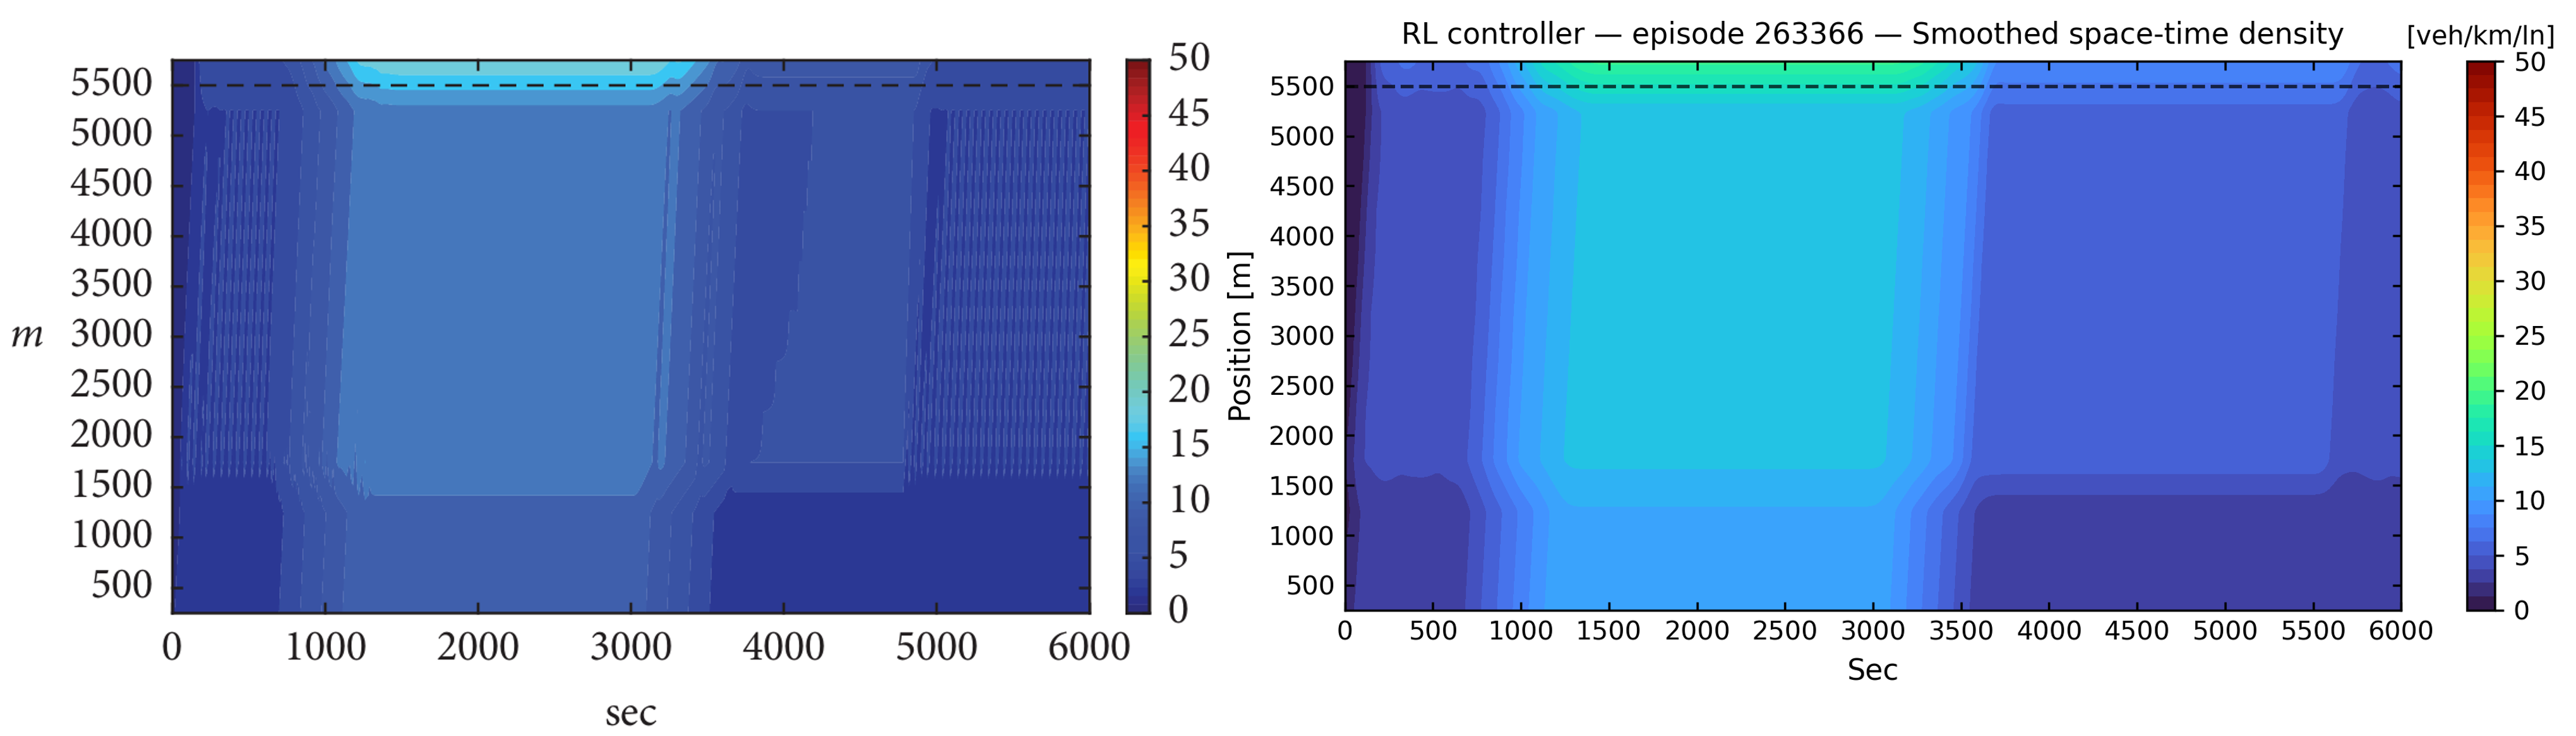
\includegraphics[width=1\linewidth]{figures/RL/final_policy/RL_space_time_density.png}
    \caption{RL-controller scenario: Space-time density contours. Original
    study (left) and reproduced result (right).}
    \label{fig:rl_spacetime}
\end{figure}


Overall, the space--time density contours in
Figure~\ref{fig:rl_spacetime} indicate that both policies produce similar, stable and
smooth traffic patterns, with densities remaining below the critical density
throughout most of the simulated freeway section. However, the control-cell
density trajectories in Figure~\ref{fig:rl_control_cell} reveal a remaining
difference between the original and reproduced controllers. The reproduced
policy appears to release excess traffic more slowly, as the control-cell
density remains above \(5\,\mathrm{veh/km/lane}\) well after \(5000\,\mathrm{s}\).

\begin{figure}[H]
    \centering
    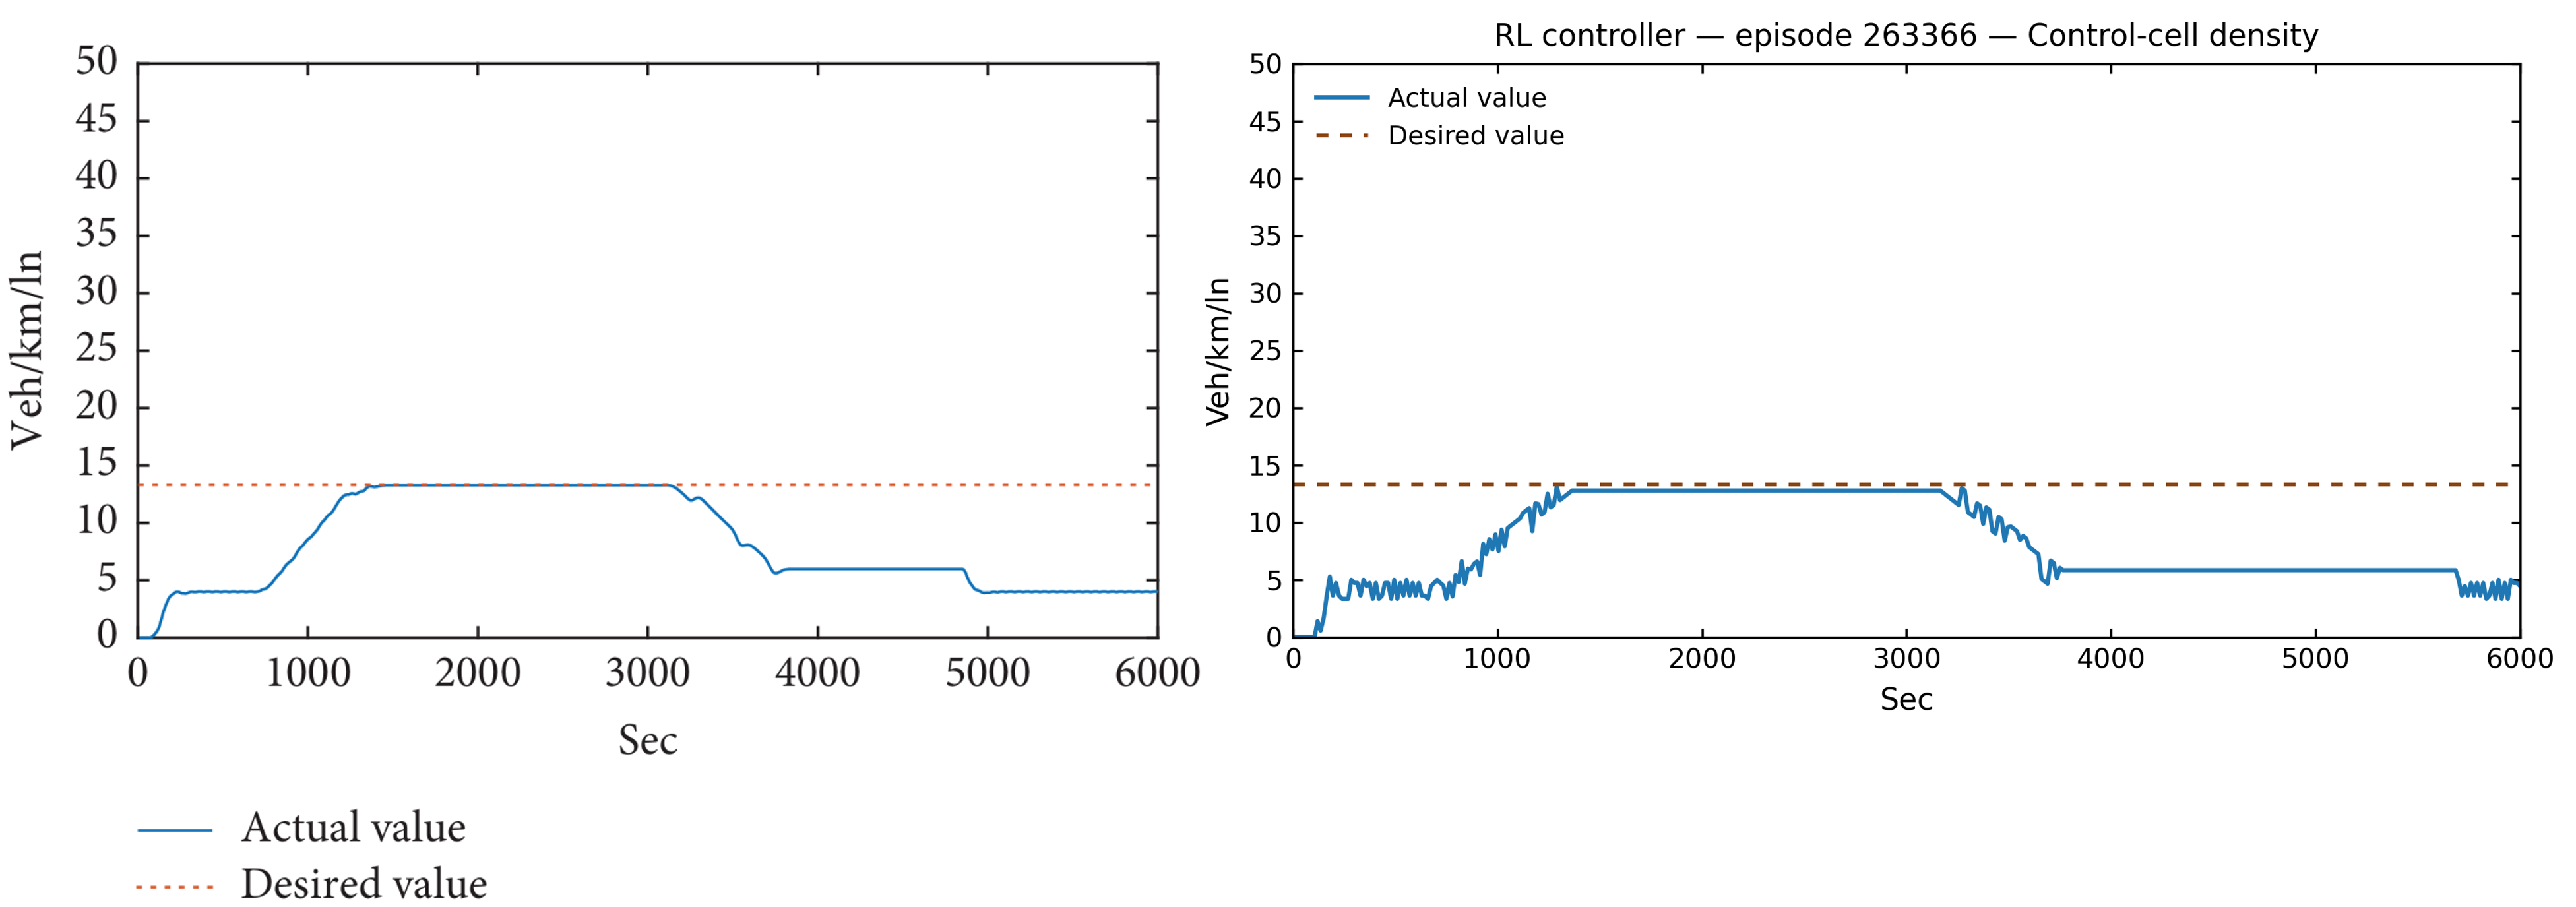
\includegraphics[width=1\linewidth]{figures/RL/final_policy/RL_control_cell_density.png}
    \caption{RL-controller scenario: control cell density. Original
    study (left) and reproduced result (right)}
    \label{fig:rl_control_cell}
\end{figure}

This interpretation is supported by the metering-rate comparison in
Figure~\ref{fig:rl_metering}. Both policies exhibit similar stable metering
intervals, but the reproduced policy is less aggressive during these intervals,
allowing a lower ramp inflow than the policy reported in the original study.
This lower release rate explains why the downstream density decreases more
slowly and remains elevated for a longer period towards the end of the
simulation.

\begin{figure}[ht]
    \centering
    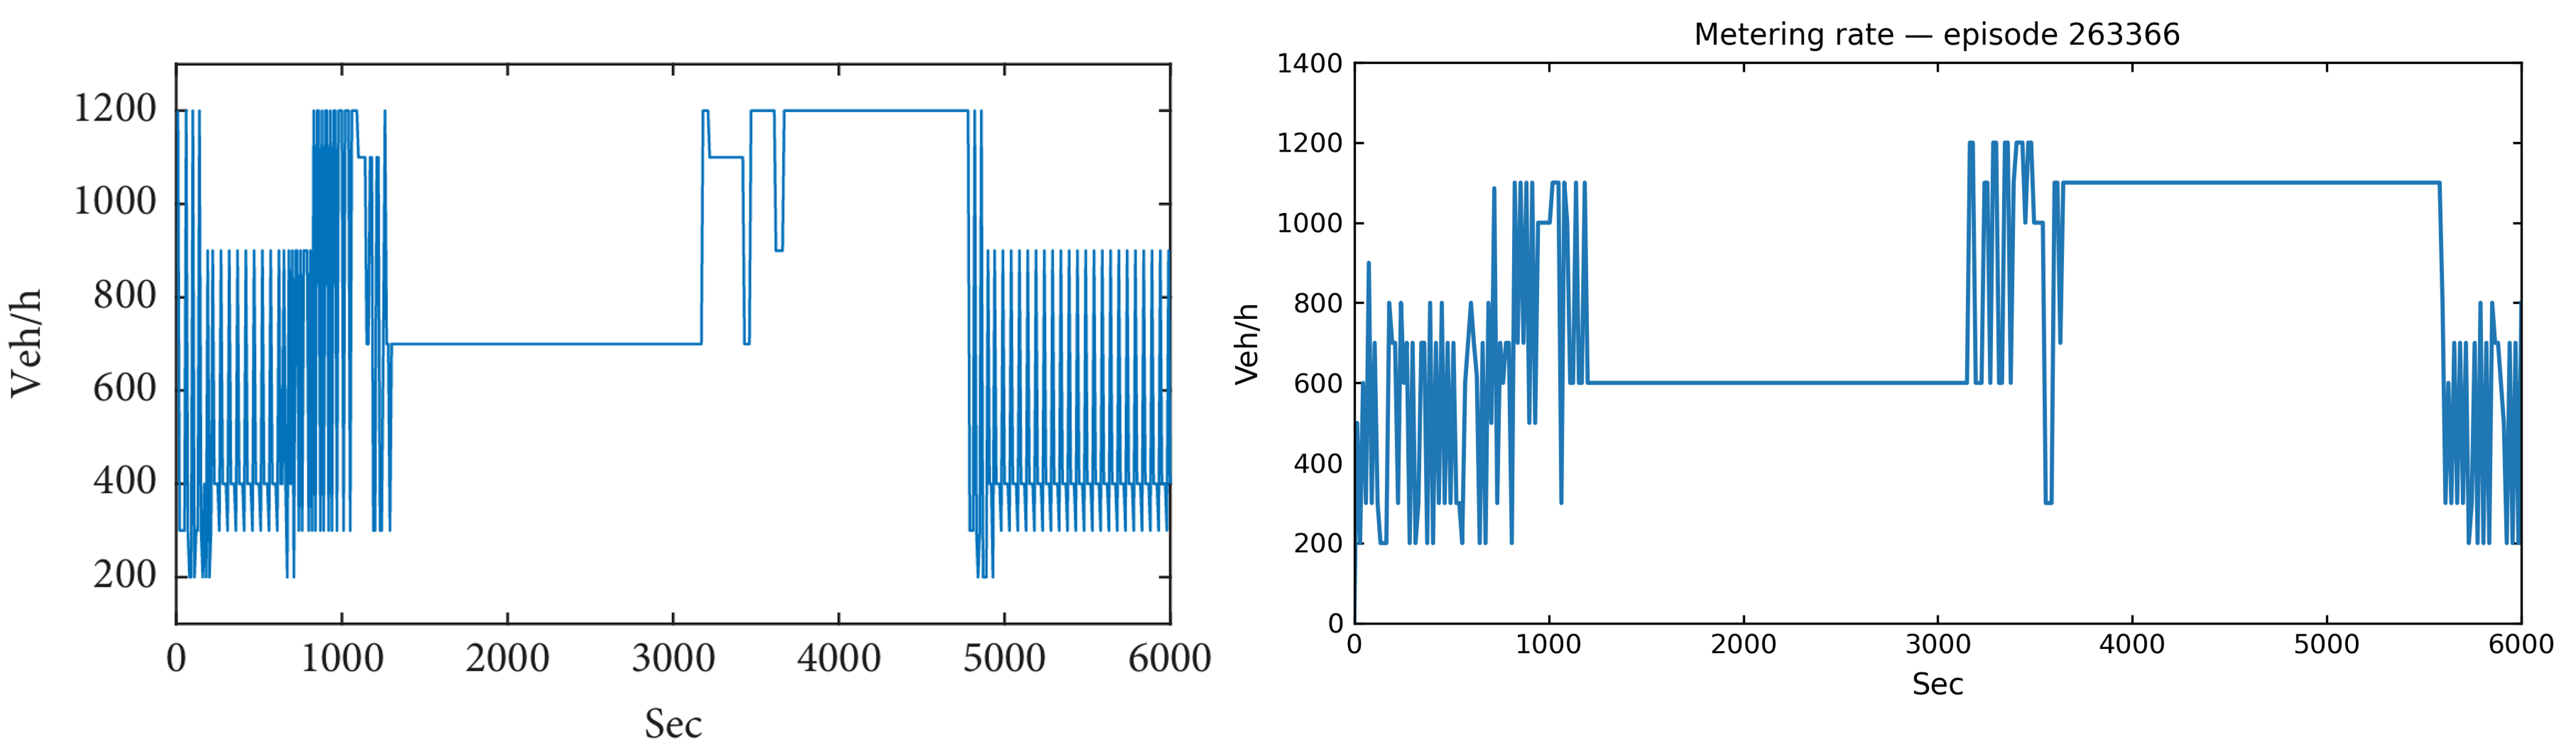
\includegraphics[width=1\linewidth]{figures/RL/final_policy/RL_metering_rate.png}
    \caption{RL-controller scenario: on-ramp metering rate. Original
    study (left) and reproduced result (right)}
    \label{fig:rl_metering}
\end{figure}

\clearpage

\subsection{Controller performance evaluation}\label{subsec:controller_perf_eval}

Table~\ref{tab:full_results} summarises the performance indicators for all controllers across the base demand scenario and five noise levels. Table~\ref{tab:rankings} reports the percentage gap of each controller relative to the best-performing controller for each indicator and demand scenario. A
value of \(0.0\%\) therefore indicates the best result within a given noise
level and performance indicator, while larger values indicate worse performance
relative to that best value. This representation makes the comparison easier to
interpret than the absolute values alone, because it shows not only which
controller performs best, but also how far the remaining controllers are from
the best observed result. This data enables a quantitative comparison of the different controllers which is absent from the original study.

Across all controllers and demand scenarios, VKT remains effectively identical (see Table \ref{tab:rankings}).
This indicates that all controllers are able to serve the same total traffic
demand over the simulation horizon and that no residual on-ramp queue remains at
the end of the episode. Consequently, differences in performance are not caused
by differences in the number of vehicles discharged from the system, but by how
efficiently these vehicles are processed over time, as reflected by VHT,
\(\mathrm{VHT}_{\mathrm{queue}}\), \(\bar{v}\), and
\(\bar{v}_{\mathrm{queue}}\). The small discrepancies observed in the RL controller's VKT across noise scenarios (see Table \ref{tab:full_results}) are attributable to its finite discrete action space, which prevents exact matching of the ramp demand at every time step and leads to the formation of negligible residual queues.

\begin{figure}[htbp]
    \centering

    \begin{subfigure}{0.48\textwidth}
        \centering
        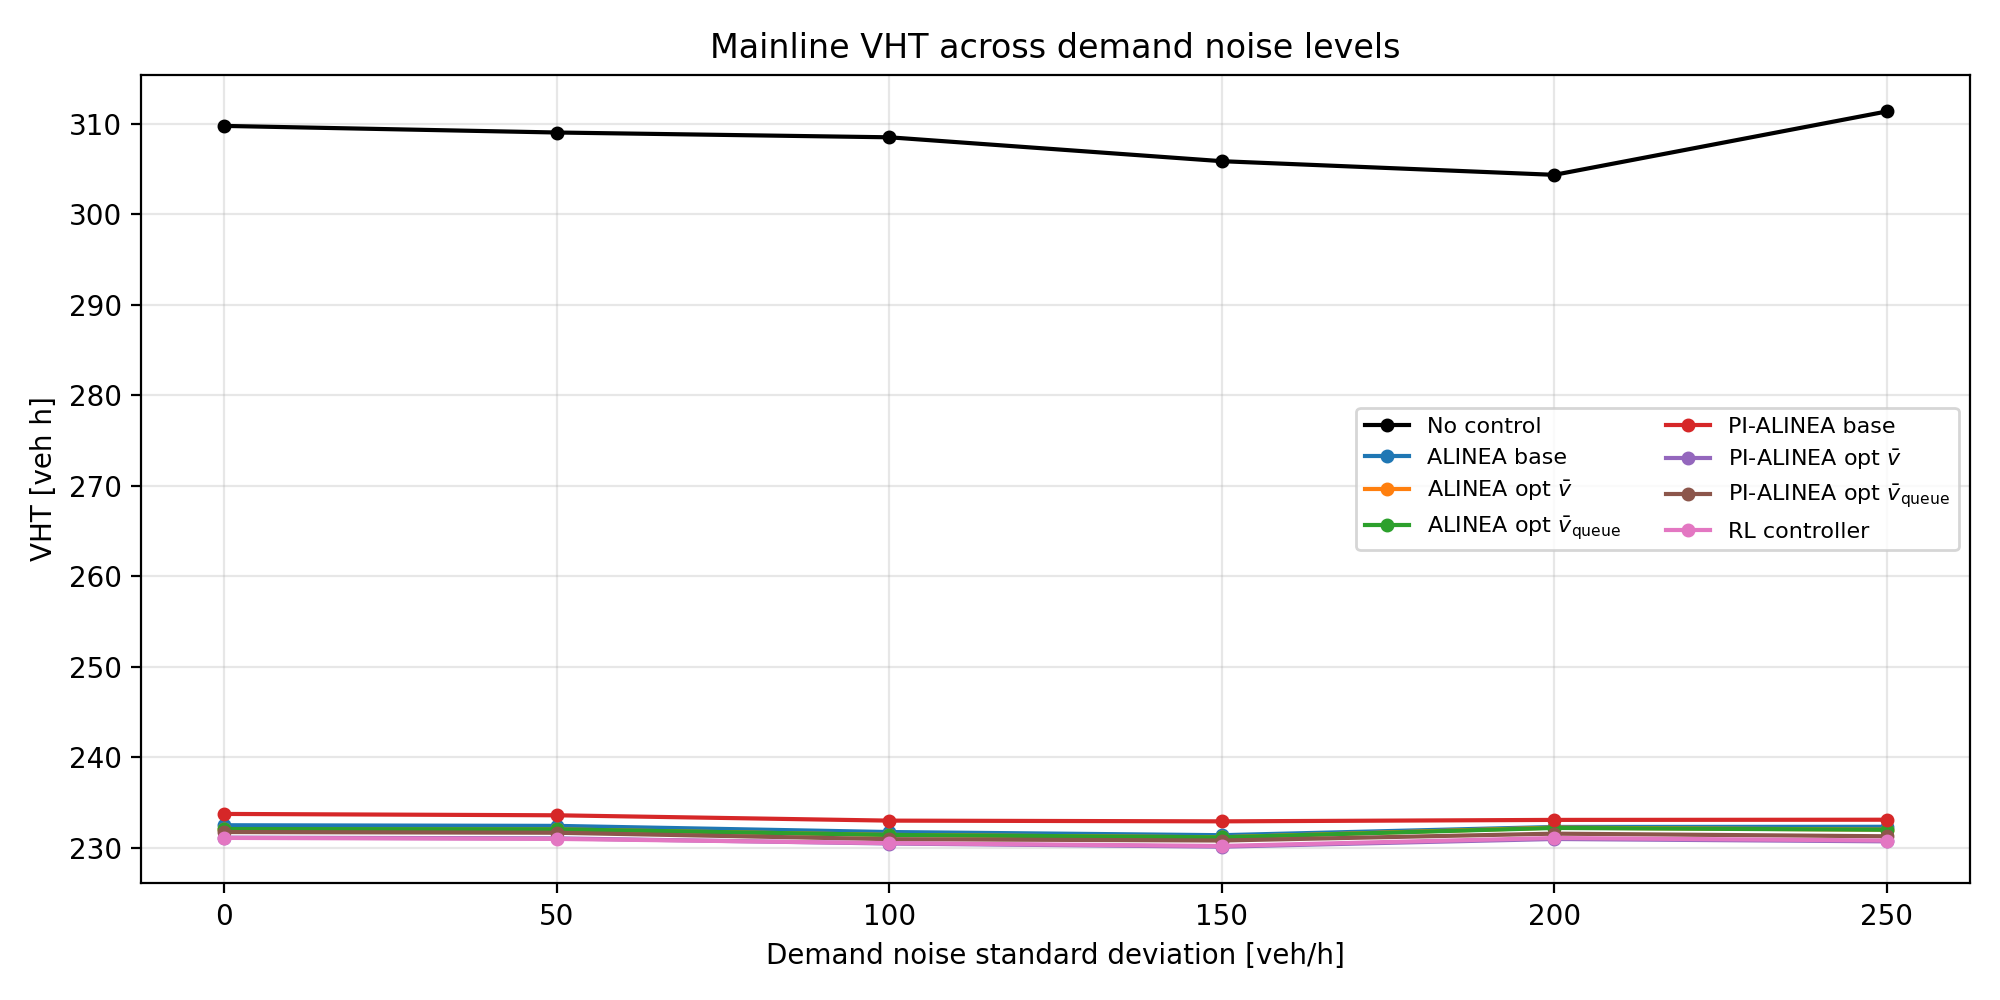
\includegraphics[width=\linewidth]{figures/Indicator_comparison/vht_vs_noise.png}
        \caption{VHT by controller, including No-control scenario}
    \end{subfigure}
    \hfill
    \begin{subfigure}{0.48\textwidth}
        \centering
        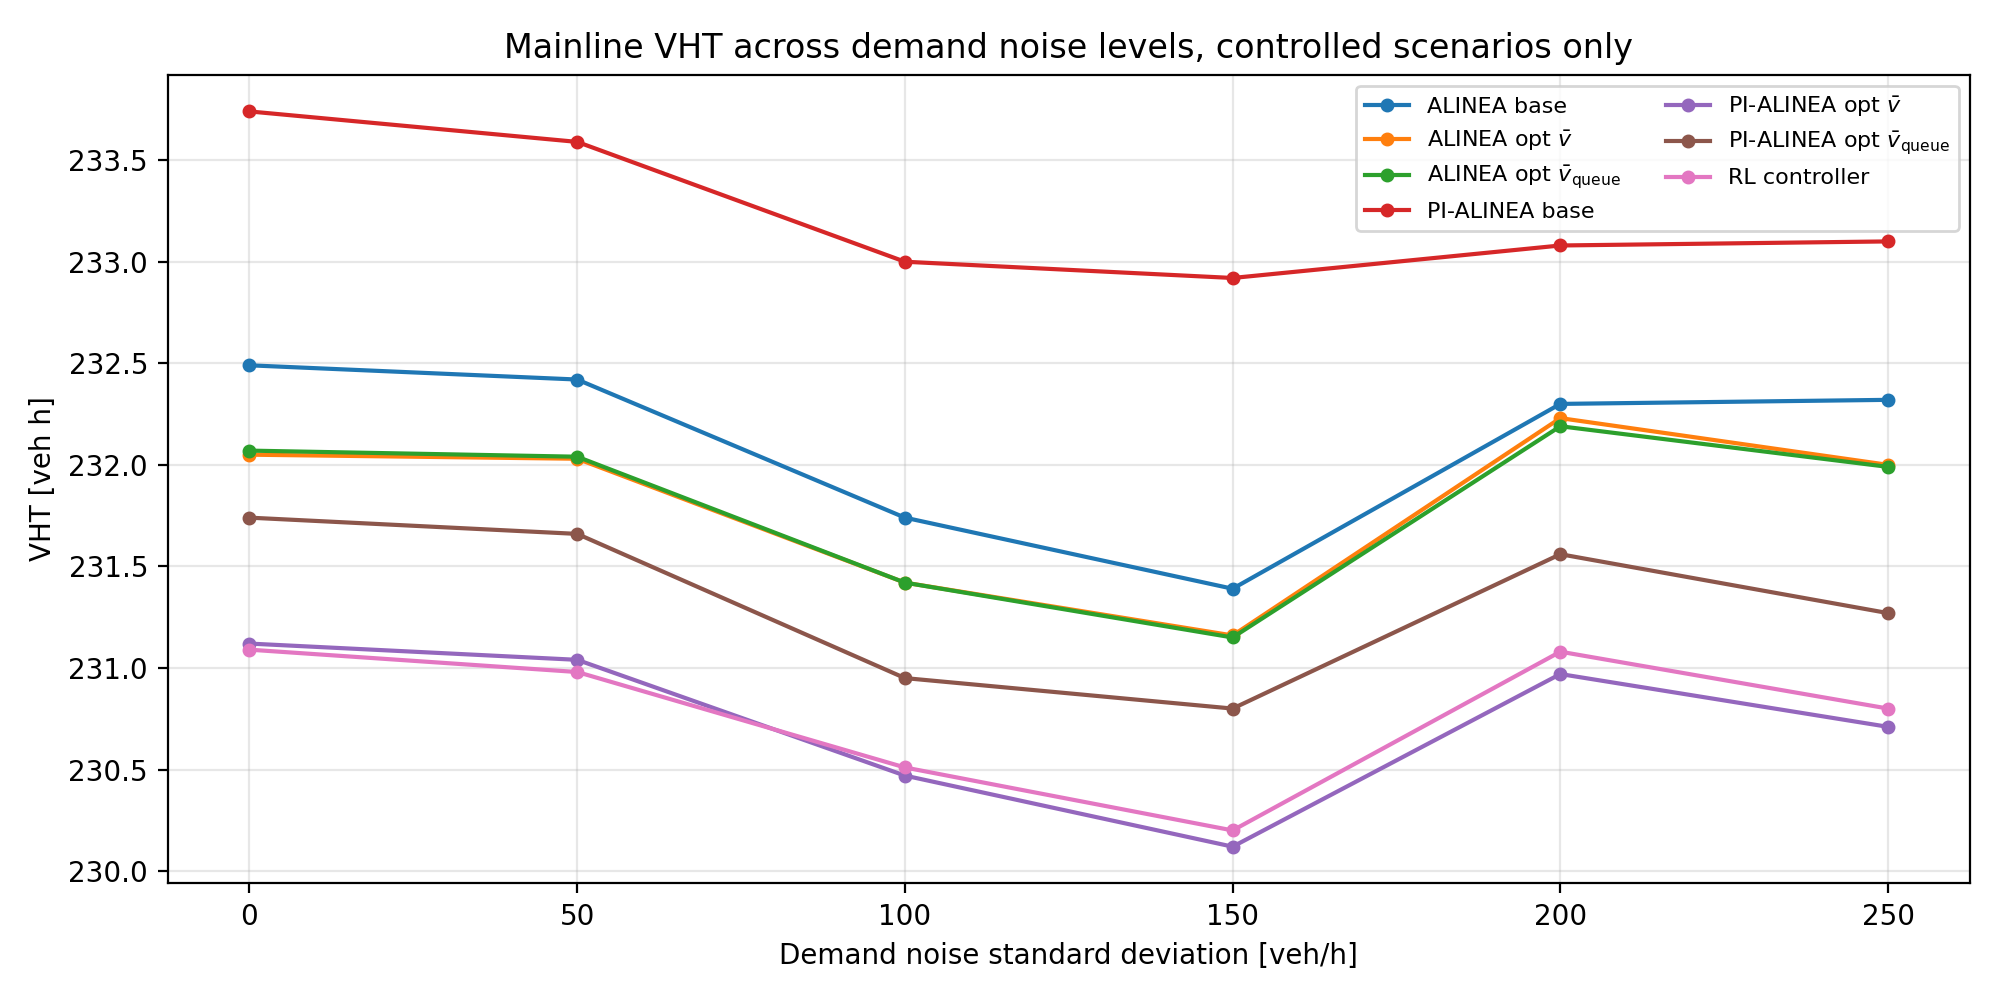
\includegraphics[width=\linewidth]{figures/Indicator_comparison/vht_vs_noise_controlled_only.png}
        \caption{VHT by controller, without No-control scenario}
    \end{subfigure}
    \caption{Evolution of VHT by controller over increasing standard deviation of the demand}
    \label{fig:indicators_vht}
\end{figure}

Mainline travel efficiency, measured by VHT and \(\bar{v}\) without ramp queue
consideration, improves substantially under all controlled scenarios relative to
the no-control baseline (see Figure \ref{fig:indicators_vht}). The controlled scenarios achieve an approximately
\(25\%\) reduction in VHT and a \(33\%\) increase in average speed (see Table \ref{tab:rankings}). Differences
between controlled strategies are, however, minor, with all metering controllers
achieving approximately \(\bar{v} \approx 119\,\mathrm{km/h}\), regardless of
the selected gains or controller variant. This suggests that once congestion at
the bottleneck is prevented, the specific control law has only limited influence
on mainline efficiency. Non-the-less, the original PI-ALINEA controller stands out as the worst of all controllers. However, the PI-ALINEA optimised for \(\bar{v}\) either beats or matches the RL-controller across all demand scenarios.

\begin{figure}[htbp]
    \centering

    \begin{subfigure}{0.48\textwidth}
        \centering
        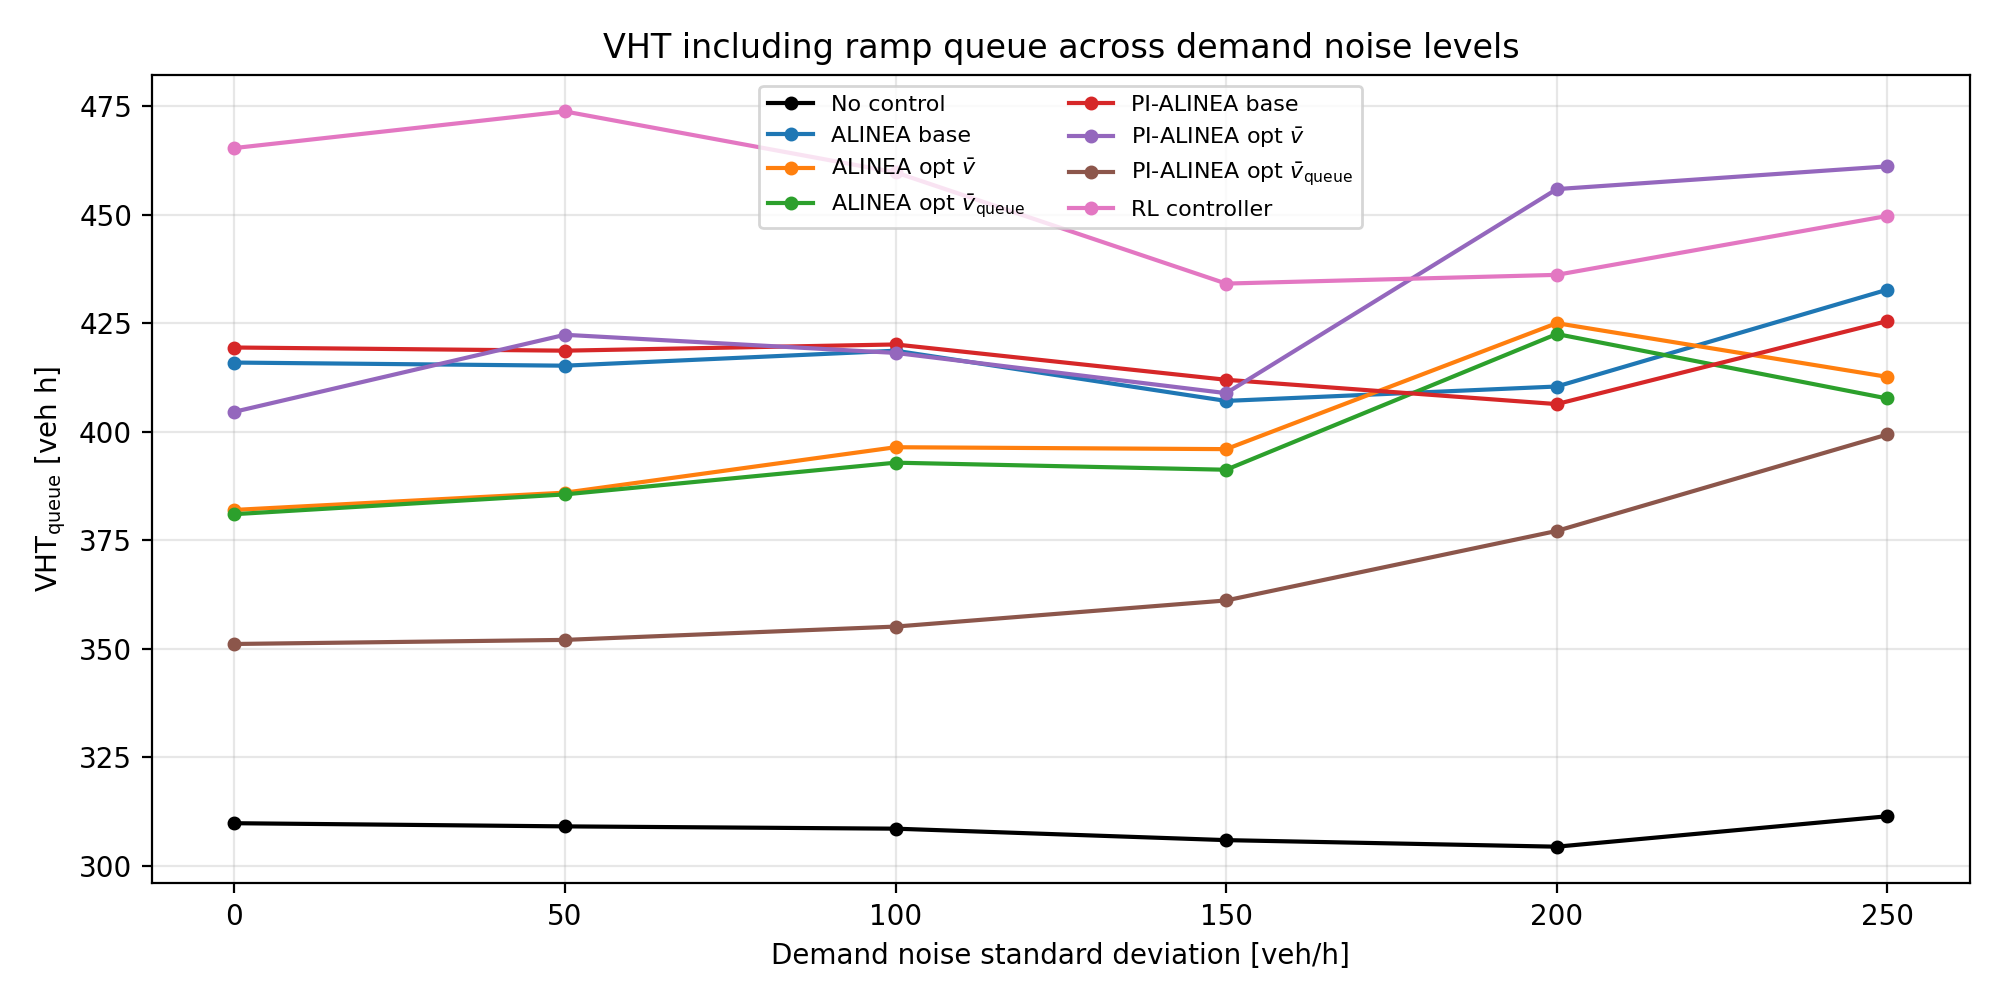
\includegraphics[width=\linewidth]{figures/Indicator_comparison/vht_queue_vs_noise.png}
        \caption{\(\mathrm{VHT}_{\mathrm{queue}}\) by controller, including No-control scenario}
    \end{subfigure}
    \hfill
    \begin{subfigure}{0.48\textwidth}
        \centering
        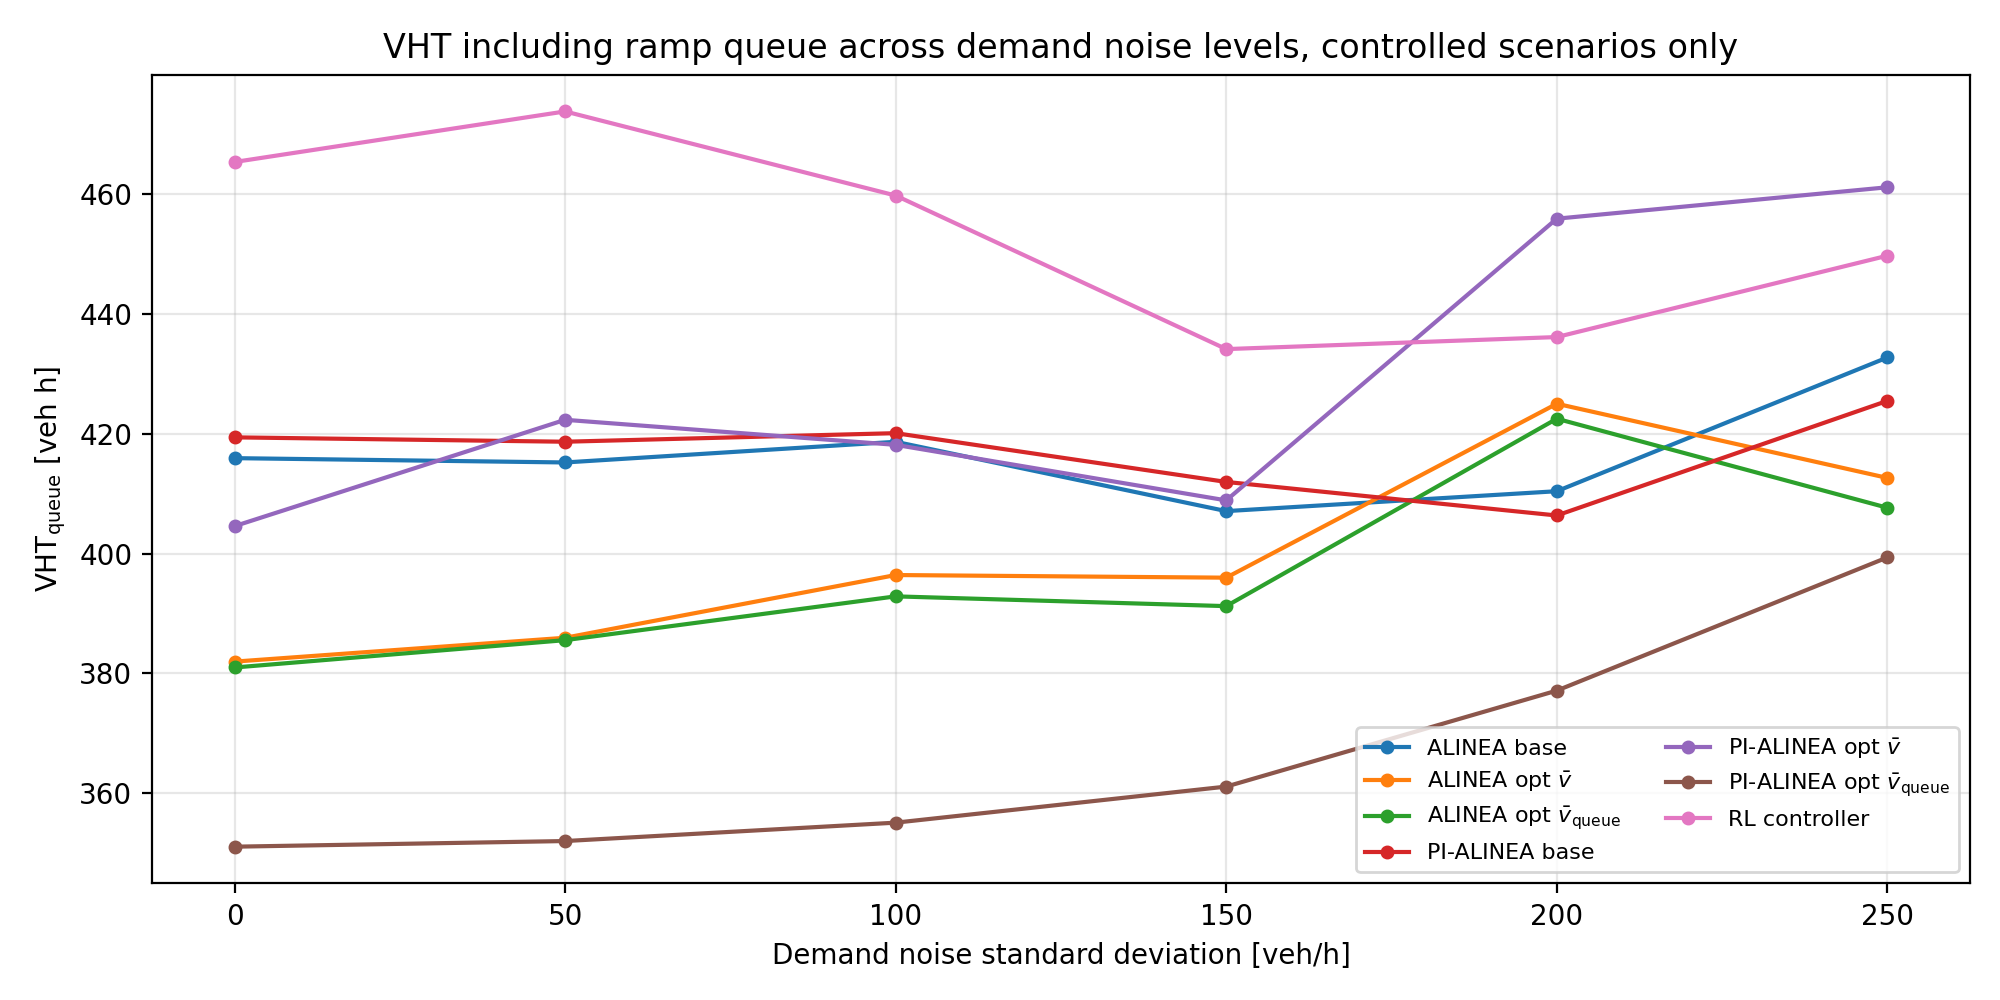
\includegraphics[width=\linewidth]{figures/Indicator_comparison/vht_queue_vs_noise_controlled_only.png}
        \caption{\(\mathrm{VHT}_{\mathrm{queue}}\) by controller, without No-control scenario}
    \end{subfigure}
    \caption{Evolution of \(\mathrm{VHT}_{\mathrm{queue}}\) by controller over increasing standard deviation of the demand}
    \label{fig:indicators_vht_queue}
\end{figure}

Figure~\ref{fig:indicators_vht_queue} shows
\(\mathrm{VHT}_{\mathrm{queue}}\) across all demand noise levels, both with and
without the no-control scenario. Compared with the mainline-only VHT results,
the queue-inclusive indicator varies much more strongly across controllers and
noise levels. While the controlled strategies differ only marginally in VHT,
small improvements in mainline travel efficiency can correspond to substantially
larger changes in \(\mathrm{VHT}_{\mathrm{queue}}\). This indicates that
optimizing directly for mainline VHT or \(\bar{v}\) alone can worsen total
system performance if the resulting policy achieves mainline stability by
holding too many vehicles on the ramp.

The no-control case performs best when queue dwelling time is included, because
it does not meter the ramp and therefore does not create an on-ramp queue. This
raises an important practical point: if the objective is defined only as total
system travel time in this reconstructed distant-bottleneck scenario, ramp
metering is not automatically favoured. However, this result must be interpreted
together with the control objective. Ramp metering is intended not only to
minimise travel time, but also to regulate mainline density, prevent bottleneck
breakdown, and stabilise traffic near the lane drop. The no-control case
performs well in \(\mathrm{VHT}_{\mathrm{queue}}\), but this comes at the
expense of poorer density tracking, as shown by the episode-reward results in
Figure~\ref{fig:indicators_reward}.

Among the controlled strategies, PI-ALINEA optimised for
\(\bar{v}_{\mathrm{queue}}\) achieves the lowest queue burden across the tested
demand scenarios. By contrast, PI-ALINEA optimised for \(\bar{v}\) achieves
excellent mainline performance but can produce considerably worse
queue-inclusive results, especially under higher demand noise. This highlights
that marginal gains in mainline VHT are not necessarily meaningful when they are
obtained by transferring delay to the on-ramp. The RL controller shows a similar
trade-off: it generally produces one of the largest queue burdens among the
metered controllers, approximately \(32\%\) higher than the best controlled
alternative under clean demand, despite strong density-tracking performance.
This is consistent with its reward formulation, which penalises deviations of
\(\rho_3\) from \(\rho_{\mathrm{des}}\) but does not include a queue term.
Exact numerical values are reported in Table~\ref{tab:full_results}.

\begin{figure}[htbp]
    \centering

    \begin{subfigure}{0.48\textwidth}
        \centering
        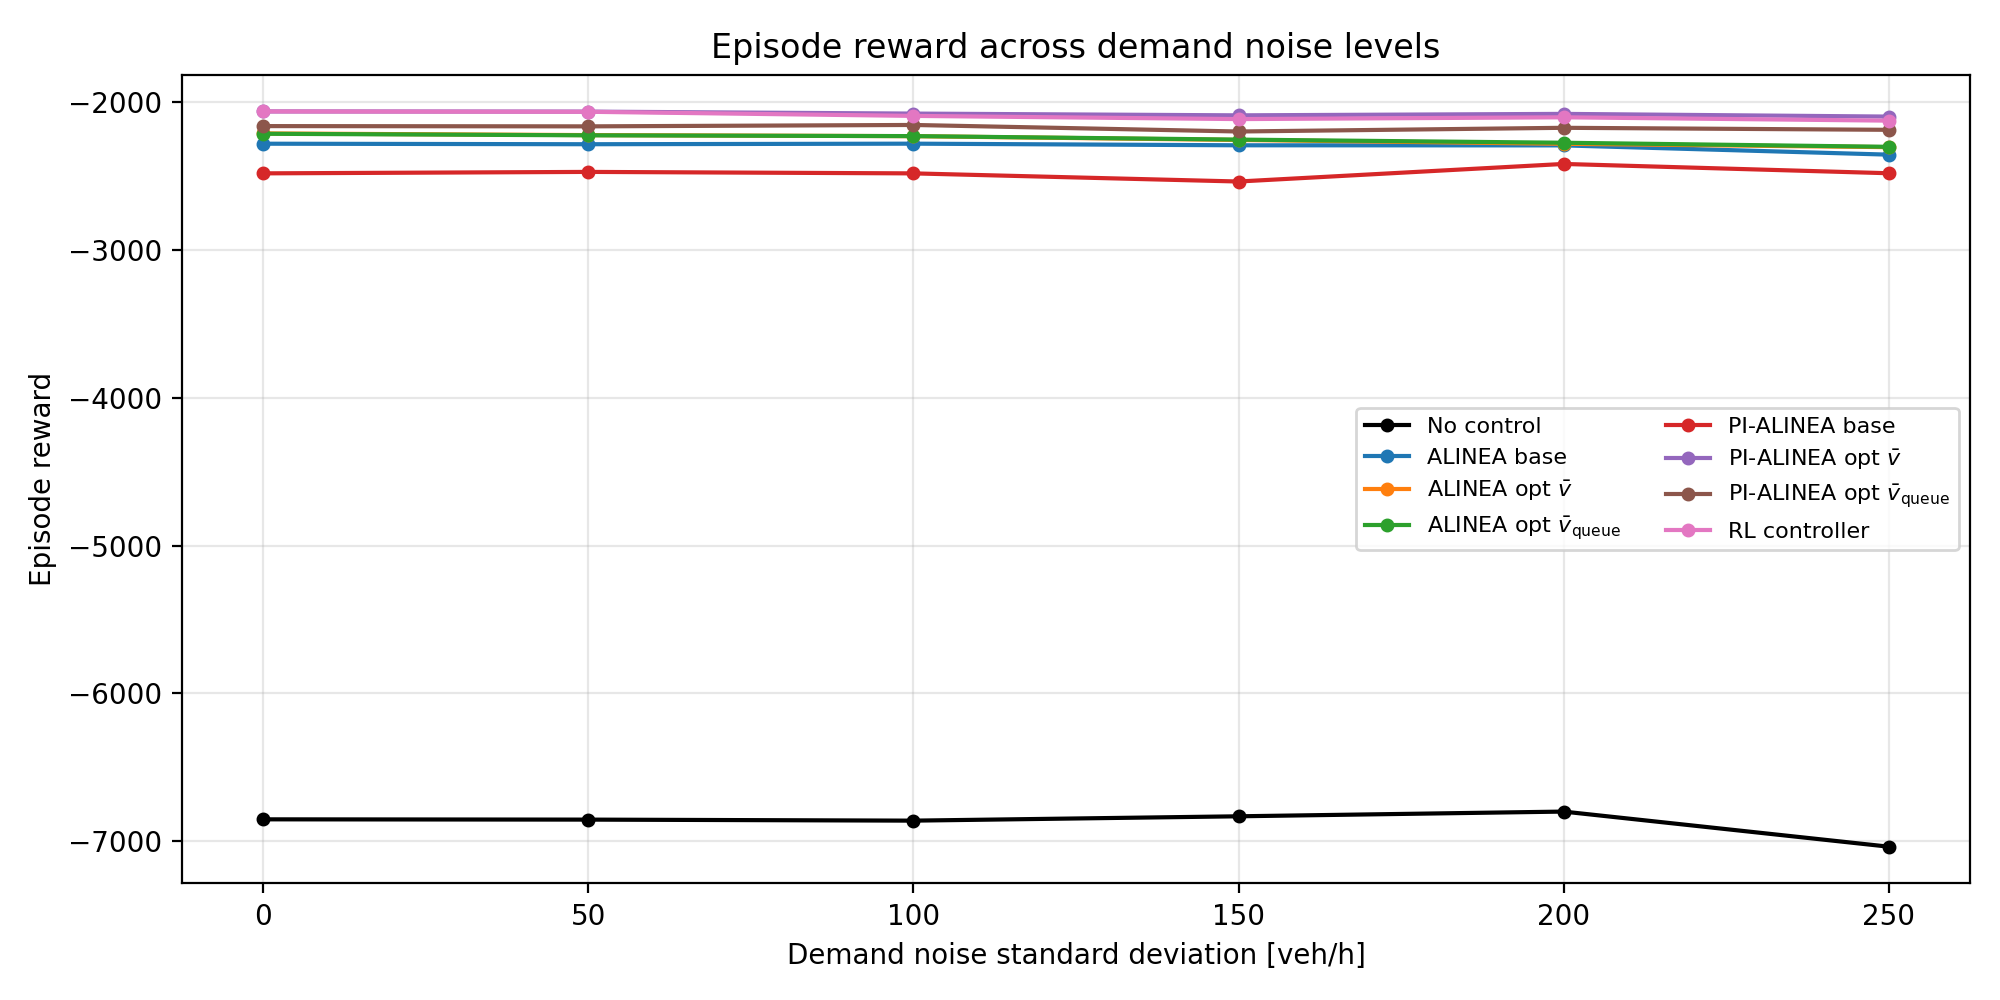
\includegraphics[width=\linewidth]{figures/Indicator_comparison/episode_reward_vs_noise.png}
        \caption{Episode reward by controller, including No-control scenario}
    \end{subfigure}
    \hfill
    \begin{subfigure}{0.48\textwidth}
        \centering
        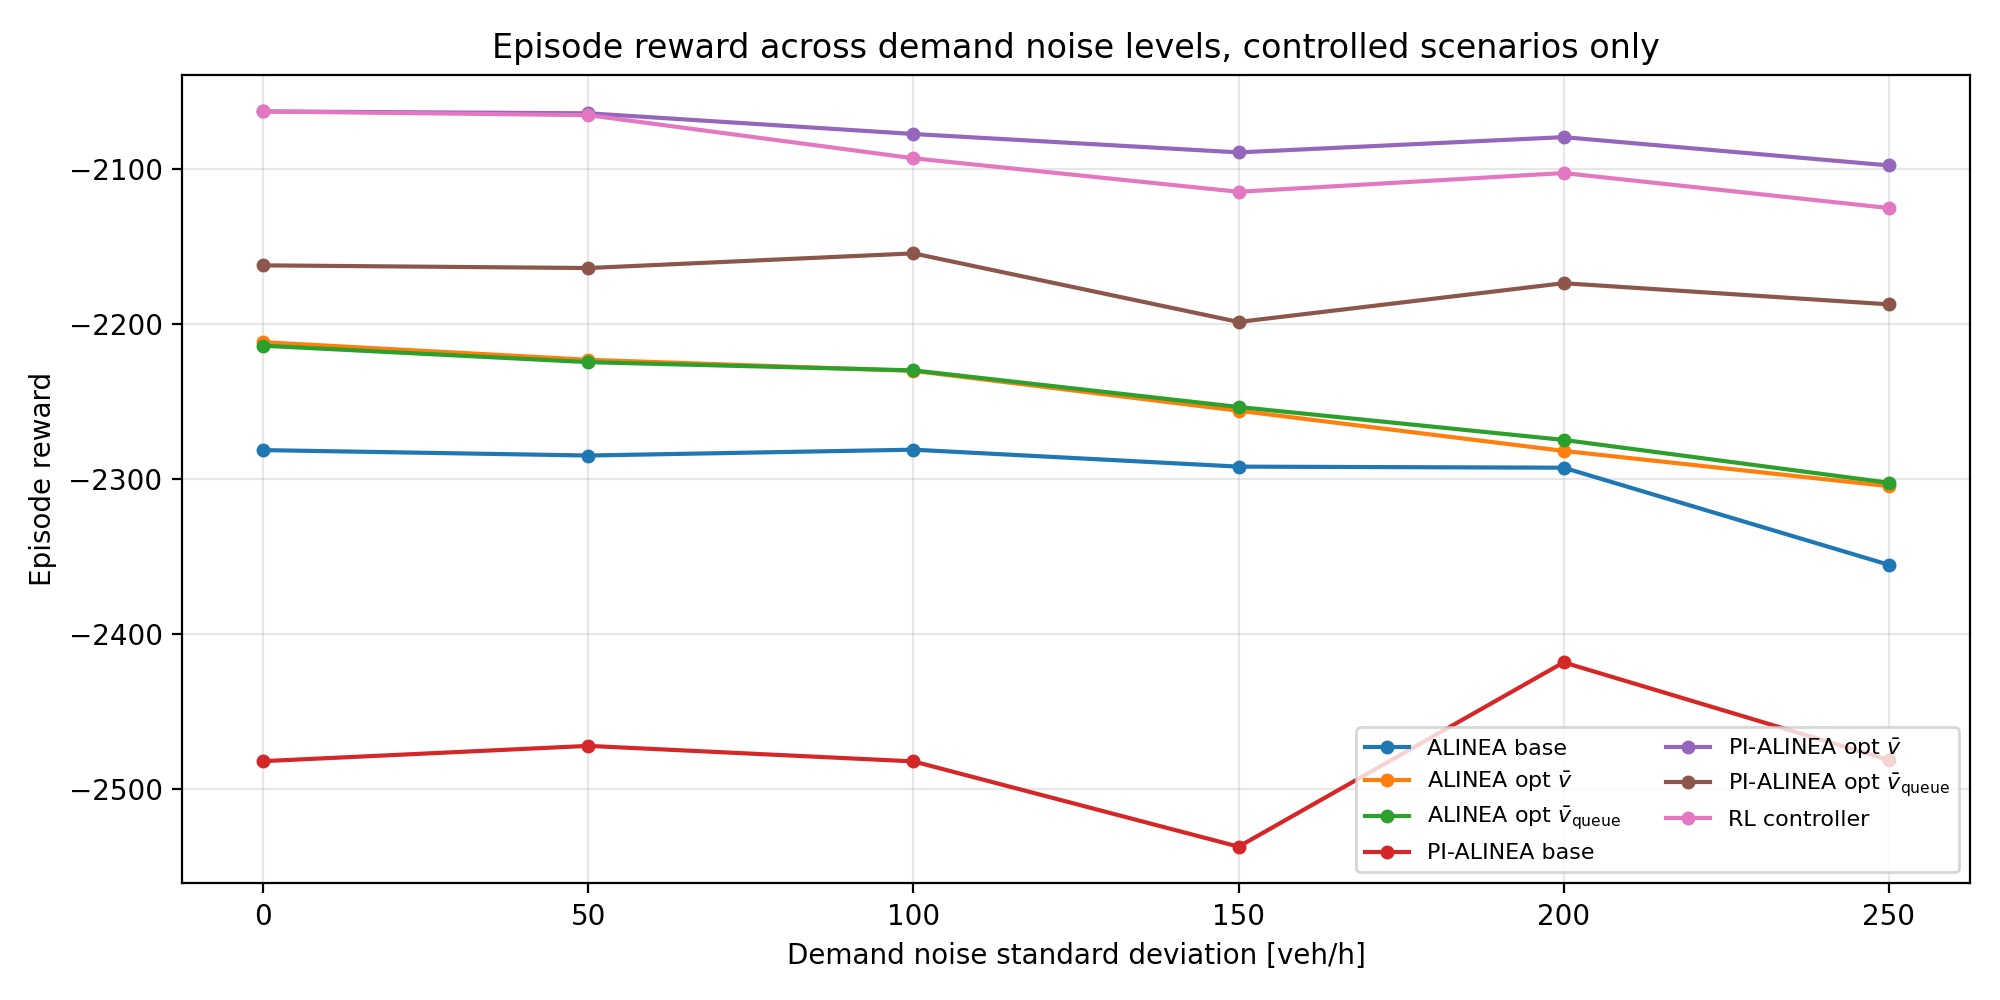
\includegraphics[width=\linewidth]{figures/Indicator_comparison/episode_reward_vs_noise_controlled_only.png}
        \caption{Episode reward by controller, without No-control scenario}
    \end{subfigure}
    \caption{Evolution of episode reward by controller over increasing standard deviation of the demand}
    \label{fig:indicators_reward} 
\end{figure}

Figure~\ref{fig:indicators_reward} compares the episode reward across demand
noise levels, both including and excluding the no-control scenario. Since the
reward directly penalises deviations of the control-cell density from
\(\rho_{\mathrm{des}}\), higher values indicate better tracking performance.

The no-control scenario performs substantially worse than all controlled
strategies, confirming that ramp metering is effective at regulating the
control-cell density. Among the controlled scenarios, the RL controller and
PI-ALINEA optimised for \(\bar{v}\) achieve the best rewards under clean demand.
Across increasing noise levels, both remain among the strongest performers,
although PI-ALINEA optimised for \(\bar{v}\) slightly outperforms the RL
controller at higher noise levels. The original PI-ALINEA parameterisation
performs clearly worse than the optimised variants, confirming the benefit of
retuning the benchmark controller. Exact indicator values can be found in Table \ref{tab:full_results}.

%\clearpage

% Required packages in the preamble:
% \usepackage{pdflscape}
% \usepackage{longtable}
% \usepackage{booktabs}
% \usepackage{array}
% \usepackage{makecell}



%\begin{landscape}
%\clearpage

\begingroup
\scriptsize
\setlength{\tabcolsep}{3pt}
\renewcommand{\arraystretch}{1.12}
\begin{longtable}{p{5.2cm}rrrrrrr}
\caption{Percentage gap from best-performing controller per indicator and demand scenario. 0.0\% indicates the best result; higher values indicate worse performance.}\label{tab:rankings}\\
\toprule
\textbf{Controller} & \makecell{\textbf{Noise std}\\\textbf{veh/h}} & \makecell{\textbf{VKT}\\\textbf{veh$\cdot$km}} & \makecell{\textbf{VHT}\\\textbf{veh$\cdot$h}} & \makecell{VHT$_{\mathrm{queue}}$\\\textbf{veh$\cdot$h}} & \makecell{\textbf{$\bar{v}$}\\\textbf{km/h}} & \makecell{\textbf{$\bar{v}_{\mathrm{queue}}$}\\\textbf{km/h}} & \makecell{\textbf{Episode}\\\textbf{reward}} \\
\midrule
\endfirsthead
\caption[]{Percentage gap from best-performing controller (continued)}\\
\toprule
Controller & \makecell{Noise std\\veh/h} & \makecell{VKT\\veh$\cdot$km} & \makecell{VHT\\veh$\cdot$h} & \makecell{VHT$_{\mathrm{queue}}$\\veh$\cdot$h} & \makecell{$\bar{v}$\\km/h} & \makecell{$\bar{v}_{\mathrm{queue}}$\\km/h} & \makecell{Episode\\reward} \\
\midrule
\endhead
\midrule
\multicolumn{8}{r}{Continued on next page}\\
\endfoot
\bottomrule
\endlastfoot
No control & 0 & 0.0\% & 34.1\% & 0.0\% & 25.4\% & 0.0\% & 232.2\% \\
ALINEA ($K_R$=10) & 0 & 0.0\% & 0.6\% & 34.3\% & 0.6\% & 25.5\% & 10.6\% \\
ALINEA opt $\bar{v}$ ($K_R$=23) & 0 & 0.0\% & 0.4\% & 23.3\% & 0.4\% & 18.9\% & 7.2\% \\
ALINEA opt $\bar{v}_{\mathrm{queue}}$ ($K_R$=21) & 0 & 0.0\% & 0.4\% & 23.0\% & 0.4\% & 18.7\% & 7.3\% \\
PI-ALINEA ($K_R$=100, $K_P$=4) & 0 & 0.0\% & 1.1\% & 35.4\% & 1.1\% & 26.1\% & 20.3\% \\
PI-ALINEA opt $\bar{v}$ ($K_R$=2, $K_P$=93) & 0 & 0.0\% & 0.0\% & 30.6\% & 0.0\% & 23.4\% & 0.0\% \\
PI-ALINEA opt $\bar{v}_{\mathrm{queue}}$ ($K_R$=2, $K_P$=56) & 0 & 0.0\% & 0.3\% & 13.3\% & 0.3\% & 11.8\% & 4.8\% \\
RL controller (ep 263366) & 0 & 0.0\% & 0.0\% & 50.2\% & 0.0\% & 33.4\% & 0.0\% \\
\midrule
No control & 50 & 0.0\% & 33.8\% & 0.0\% & 25.2\% & 0.0\% & 232.1\% \\
ALINEA ($K_R$=10) & 50 & 0.0\% & 0.6\% & 34.3\% & 0.6\% & 25.6\% & 10.7\% \\
ALINEA opt $\bar{v}$ ($K_R$=23) & 50 & 0.0\% & 0.5\% & 24.9\% & 0.4\% & 19.9\% & 7.7\% \\
ALINEA opt $\bar{v}_{\mathrm{queue}}$ ($K_R$=21) & 50 & 0.0\% & 0.5\% & 24.8\% & 0.4\% & 19.8\% & 7.8\% \\
PI-ALINEA ($K_R$=100, $K_P$=4) & 50 & 0.0\% & 1.1\% & 35.5\% & 1.1\% & 26.2\% & 19.8\% \\
PI-ALINEA opt $\bar{v}$ ($K_R$=2, $K_P$=93) & 50 & 0.0\% & 0.0\% & 36.7\% & 0.0\% & 26.8\% & 0.0\% \\
PI-ALINEA opt $\bar{v}_{\mathrm{queue}}$ ($K_R$=2, $K_P$=56) & 50 & 0.0\% & 0.3\% & 13.9\% & 0.3\% & 12.2\% & 4.8\% \\
RL controller (ep 263366) & 50 & 0.0\% & 0.0\% & 53.3\% & 0.0\% & 34.8\% & 0.1\% \\
\midrule
No control & 100 & 0.0\% & 33.9\% & 0.0\% & 25.3\% & 0.0\% & 230.3\% \\
ALINEA ($K_R$=10) & 100 & 0.0\% & 0.6\% & 35.7\% & 0.6\% & 26.3\% & 9.8\% \\
ALINEA opt $\bar{v}$ ($K_R$=23) & 100 & 0.0\% & 0.4\% & 28.5\% & 0.4\% & 22.2\% & 7.4\% \\
ALINEA opt $\bar{v}_{\mathrm{queue}}$ ($K_R$=21) & 100 & 0.0\% & 0.4\% & 27.3\% & 0.4\% & 21.5\% & 7.3\% \\
PI-ALINEA ($K_R$=100, $K_P$=4) & 100 & 0.0\% & 1.1\% & 36.2\% & 1.1\% & 26.6\% & 19.5\% \\
PI-ALINEA opt $\bar{v}$ ($K_R$=2, $K_P$=93) & 100 & 0.0\% & 0.0\% & 35.5\% & 0.0\% & 26.2\% & 0.0\% \\
PI-ALINEA opt $\bar{v}_{\mathrm{queue}}$ ($K_R$=2, $K_P$=56) & 100 & 0.0\% & 0.2\% & 15.1\% & 0.2\% & 13.1\% & 3.7\% \\
RL controller (ep 263366) & 100 & 0.0\% & 0.0\% & 49.0\% & 0.0\% & 32.9\% & 0.8\% \\
\midrule
No control & 150 & 0.0\% & 32.9\% & 0.0\% & 24.8\% & 0.0\% & 227.0\% \\
ALINEA ($K_R$=10) & 150 & 0.0\% & 0.6\% & 33.1\% & 0.5\% & 24.9\% & 9.7\% \\
ALINEA opt $\bar{v}$ ($K_R$=23) & 150 & 0.0\% & 0.5\% & 29.5\% & 0.5\% & 22.8\% & 8.0\% \\
ALINEA opt $\bar{v}_{\mathrm{queue}}$ ($K_R$=21) & 150 & 0.0\% & 0.4\% & 27.9\% & 0.4\% & 21.8\% & 7.9\% \\
PI-ALINEA ($K_R$=100, $K_P$=4) & 150 & 0.0\% & 1.2\% & 34.7\% & 1.2\% & 25.7\% & 21.4\% \\
PI-ALINEA opt $\bar{v}$ ($K_R$=2, $K_P$=93) & 150 & 0.0\% & 0.0\% & 33.7\% & 0.0\% & 25.2\% & 0.0\% \\
PI-ALINEA opt $\bar{v}_{\mathrm{queue}}$ ($K_R$=2, $K_P$=56) & 150 & 0.0\% & 0.3\% & 18.1\% & 0.3\% & 15.3\% & 5.2\% \\
RL controller (ep 263366) & 150 & 0.0\% & 0.0\% & 41.9\% & 0.1\% & 29.6\% & 1.2\% \\
\midrule
No control & 200 & 0.0\% & 31.8\% & 0.0\% & 24.1\% & 0.0\% & 227.0\% \\
ALINEA ($K_R$=10) & 200 & 0.0\% & 0.6\% & 34.8\% & 0.6\% & 25.8\% & 10.3\% \\
ALINEA opt $\bar{v}$ ($K_R$=23) & 200 & 0.0\% & 0.5\% & 39.6\% & 0.5\% & 28.4\% & 9.7\% \\
ALINEA opt $\bar{v}_{\mathrm{queue}}$ ($K_R$=21) & 200 & 0.0\% & 0.5\% & 38.8\% & 0.5\% & 28.0\% & 9.4\% \\
PI-ALINEA ($K_R$=100, $K_P$=4) & 200 & 0.0\% & 0.9\% & 33.5\% & 0.9\% & 25.1\% & 16.3\% \\
PI-ALINEA opt $\bar{v}$ ($K_R$=2, $K_P$=93) & 200 & 0.0\% & 0.0\% & 49.8\% & 0.0\% & 33.2\% & 0.0\% \\
PI-ALINEA opt $\bar{v}_{\mathrm{queue}}$ ($K_R$=2, $K_P$=56) & 200 & 0.0\% & 0.3\% & 23.9\% & 0.3\% & 19.3\% & 4.5\% \\
RL controller (ep 263366) & 200 & 0.0\% & 0.0\% & 43.3\% & 0.1\% & 30.2\% & 1.1\% \\
\midrule
No control & 250 & 0.0\% & 35.0\% & 0.0\% & 25.9\% & 0.0\% & 235.5\% \\
ALINEA ($K_R$=10) & 250 & 0.0\% & 0.7\% & 39.0\% & 0.7\% & 28.0\% & 12.3\% \\
ALINEA opt $\bar{v}$ ($K_R$=23) & 250 & 0.0\% & 0.6\% & 32.5\% & 0.6\% & 24.5\% & 9.9\% \\
ALINEA opt $\bar{v}_{\mathrm{queue}}$ ($K_R$=21) & 250 & 0.0\% & 0.6\% & 30.9\% & 0.6\% & 23.6\% & 9.8\% \\
PI-ALINEA ($K_R$=100, $K_P$=4) & 250 & 0.0\% & 1.0\% & 36.6\% & 1.0\% & 26.8\% & 18.3\% \\
PI-ALINEA opt $\bar{v}$ ($K_R$=2, $K_P$=93) & 250 & 0.0\% & 0.0\% & 48.1\% & 0.0\% & 32.5\% & 0.0\% \\
PI-ALINEA opt $\bar{v}_{\mathrm{queue}}$ ($K_R$=2, $K_P$=56) & 250 & 0.0\% & 0.2\% & 28.3\% & 0.2\% & 22.0\% & 4.3\% \\
RL controller (ep 263366) & 250 & 0.0\% & 0.0\% & 44.4\% & 0.1\% & 30.8\% & 1.3\% \\
\end{longtable}
%\end{landscape}
\endgroup

\clearpage

\subsection{Discussion}

The reproduction confirms that the main simulation environment can be
reconstructed with high fidelity. In particular, the no-control scenario and the
reference PI-ALINEA scenario show close agreement with the figures reported in
the original article. This suggests that the selected CTM discretisation,
boundary conditions, demand profile, and lane-drop representation are sufficiently
consistent with the original experimental setup.

However, the central performance claim of the original study is only partially
supported. The reproduced RL controller achieves stable control-cell density
tracking and smooth space--time density patterns, which is consistent with the
qualitative behaviour reported by the authors. The original article describes the
learned policy as maintaining the control target density close to the desired
value with almost no fluctuations and showing some robustness under uncertain
demands. Nevertheless, when compared against optimised benchmark controllers,
the RL controller does not provide a clear advantage. In the reconstructed
experiments, PI-ALINEA optimised for \(\bar{v}\) matches or slightly outperforms
the RL controller in mainline efficiency and episode reward, while PI-ALINEA
optimised for \(\bar{v}_{\mathrm{queue}}\) performs substantially better when
ramp queueing time is included.

This result highlights the importance of benchmark calibration. The original
study compares the proposed RL controller only against one PI-ALINEA
parameterisation. In this reproduction, the same PI-ALINEA configuration was
successfully reproduced, but the grid search showed that it is not the strongest
available benchmark for the reconstructed environment. This makes the comparison
with the RL controller sensitive to the choice of benchmark parameters. Once the
benchmark controller is retuned, the RL policy appears less like a fundamentally
superior control strategy and more like a slightly less queue-aware version of an
optimised PI-ALINEA controller.

A second limitation concerns the reward design. The RL reward penalises only the
deviation of the control-cell density \(\rho_3\) from the desired density
\(\rho_{\mathrm{des}}\). It therefore encourages density tracking at the
downstream bottleneck, but does not directly penalise ramp queueing delay. This
explains why the RL controller performs well in terms of episode reward and
mainline VHT, but poorly in terms of
\(\mathrm{VHT}_{\mathrm{queue}}\). This is not necessarily a failure of the
learning algorithm; rather, it reflects the objective that the agent was trained
to optimise. The original authors themselves identify ramp queue management as a
future extension, explicitly suggesting that queue length should be managed at
the cost of some mainline efficiency.

The training setup also limits the interpretation of the learned policy. The ANN
was trained on a single reconstructed demand profile, while robustness was
evaluated only afterwards by adding demand noise. As a result, the trained policy
may partly exploit regularities of this specific demand pattern rather than
learning a broadly generalisable ramp-metering strategy. Training directly on
randomised or noisy demand profiles would likely provide a more meaningful test
of generalisation. In particular, demand perturbations could stimulate regions of
the state space that are never visited under the deterministic base demand. For
example, the ramp-demand encoding includes bins below \(500\,\mathrm{veh/h}\),
although the deterministic ramp demand never falls below this value during
training. Under sufficiently noisy demand, these bins may become active, allowing
the agent to learn responses to states that are otherwise unused.

Finally, the reproduction was affected by several missing implementation details.
The original article does not report the CTM discretisation parameters
\(\Delta x\) and \(\Delta t\), the demand profile numerically, the
\(\epsilon\)-decay schedule, the convergence criterion, the reward scaling
constant, the network initialisation procedure, or the exact figure smoothing
procedure. These omissions required several reconstruction choices and
post-hoc checks. While the resulting baseline reproduction is visually close to
the published figures, exact reproducibility remains limited. This supports the
broader concern that transportation simulation studies require more complete
reporting of source code, demand data, calibration procedures, and controller
parameters.

\clearpage